\documentclass[12pt]{article}





\usepackage{hyperref}
\usepackage{listings}
\usepackage{xcolor}
%for json
\usepackage{bera}% optional: just to have a nice mono-spaced font
\usepackage{xcolor}
\colorlet{punct}{red!60!black}
\definecolor{background}{HTML}{EEEEEE}
\definecolor{delim}{RGB}{20,105,176}
\colorlet{numb}{magenta!60!black}
\lstdefinelanguage{json}{
	basicstyle=\normalfont\ttfamily,
	numbers=left,
	numberstyle=\scriptsize,
	stepnumber=1,
	numbersep=8pt,
	showstringspaces=false,
	breaklines=true,
	frame=lines,
	backgroundcolor=\color{background},
	literate=
	*{0}{{{\color{numb}0}}}{1}
	{1}{{{\color{numb}1}}}{1}
	{2}{{{\color{numb}2}}}{1}
	{3}{{{\color{numb}3}}}{1}
	{4}{{{\color{numb}4}}}{1}
	{5}{{{\color{numb}5}}}{1}
	{6}{{{\color{numb}6}}}{1}
	{7}{{{\color{numb}7}}}{1}
	{8}{{{\color{numb}8}}}{1}
	{9}{{{\color{numb}9}}}{1}
	{:}{{{\color{punct}{:}}}}{1}
	{,}{{{\color{punct}{,}}}}{1}
	{\{}{{{\color{delim}{\{}}}}{1}
	{\}}{{{\color{delim}{\}}}}}{1}
	{[}{{{\color{delim}{[}}}}{1}
	{]}{{{\color{delim}{]}}}}{1},
}




%for bash 

\usepackage{listings}
\usepackage{color}

\definecolor{codegreen}{rgb}{0,0.6,0}
\definecolor{codegray}{rgb}{0.5,0.5,0.5}
\definecolor{codepurple}{rgb}{0.58,0,0.82}
\definecolor{backcolour}{rgb}{0.95,0.95,0.92}


\lstset{frame=tb,
	backgroundcolor=\color{white},   
	commentstyle=\color{codegreen},
	keywordstyle=\color{magenta},
	numberstyle=\tiny\color{codegray},
	stringstyle=\color{codepurple},
	basicstyle=\footnotesize,
	breakatwhitespace=false,         
	breaklines=true,                 
	captionpos=b,                    
	keepspaces=true,                 
	numbers=left,                    
	numbersep=5pt,                  
	showspaces=false,                
	showstringspaces=false,
	showtabs=false,                  
	tabsize=2
}
\lstset{language=sh}

\usepackage{subfig}
\usepackage[utf8]{inputenc} % Required for inputting international characters
\usepackage[T1]{fontenc} % Output font encoding for international characters
\usepackage[margin=1in]{geometry}
\usepackage{mathpazo} % Palatino font
\usepackage{array}
\usepackage{float}
\usepackage{graphicx}
\usepackage{hyperref}
\usepackage{pdfpages}
\usepackage{natbib}
\setcounter{tocdepth}{2}
\graphicspath{ {C:/Users/Silvi/OneDrive/Desktop/Individual Project/Images} }

\usepackage{fancyhdr}
\usepackage[parfill]{parskip}
\pagestyle{fancy}
\usepackage{setspace}
\onehalfspacing

\begin{document}
	
	
	% Configuring the header and footer here
	\fancyhead{} % clear all header fields
	\fancyhead[RO,LE]{\textbf{M00702000}}
	\fancyhead[LO,LE]{\textbf{Final Report}}
	\fancyfoot{} % clear all footer fields
	\fancyfoot[CO]{\thepage}
	%Header and footer configuration ends here
	\begin{titlepage}	
		\centering
		
		\newcommand{\HRule}{\rule{\linewidth}{0.7mm }} % Defines a new command for horizontal lines, change thickness here
		\newcommand{\Botline}{\rule{\linewidth}{0.4mm }} % Defines a new command for horizontal lines, change thickness here
		
		
		
\includegraphics[width=0.5\linewidth]{mdx.jpg}
		%		\textsc{\LARGE Institution Name}\\[1.5cm] % Main heading such as the name of your university/college
		
		\textsc{\Large Individual Project }\\[0.5cm] % Major heading such as course name
		
		\textsc{\large Final Report}\\[0.5cm] % Minor heading such as course title
		
		%------------------------------------------------
		%	Title
		%------------------------------------------------
		
		\HRule\\[0.4cm]
		
		{\huge\bfseries Deploying And Examining Security Onion For Network Threat Detection In A Simulated Network Environment}\\[0.4cm] % Title of your document
		
		\Botline\\[1.5cm]
		
		%------------------------------------------------
		%	Author(s)
		%------------------------------------------------
		
		\begin{minipage}{0.4\textwidth}
			\begin{flushleft}
				\large
				\textit{Author}\\
				Silvia Aminul 
			\end{flushleft}
		\end{minipage}
		~
		\begin{minipage}{0.4\textwidth}
			\begin{flushright}
				\large
				\textit{Supervisor}\\
				Dr. Kamran Ali  
			\end{flushright}
			
			
		\end{minipage}
		
		
		\vfill\vfill\vfill
		
		\vfill
		%  	{\bfseries The author of this proposal \\  }
		
		
		
		{\bfseries M00702000 }
		\vfill
		{\large\today}
	\end{titlepage}	
	\newpage
	\section{Abstract}
	The objective of this project revolves around determining the effectiveness of Security Onion as an operating system specialised in threat detection. To address this, this project involves carrying out the necessary research and evaluating the deployment of Security Onion by injecting low-risk threats in a controlled environment. The results of this deployment are examined though observing the system's health performance and security logs. The insight gained from evaluating the findings indicates that Security Onion's default configurations fulfill the need for an efficient system, and although this may not cater to everyone it is an effective configuration for first-time users to gain familiarity with the system's functionality. A further note to be made based on the previous statement is that the documentation for Security Onion has a broad guide and therefore the system configurations can be manipulated to accommodate various needs.
	\newpage
	
	\tableofcontents
	\newpage
	
	
	
	\newgeometry{margin=2.5cm} % Adjust the margin value as needed
	
	\begin{center}
		
		
		\vspace*{\fill}
		
		\textbf{Declaration of Authenticity}
		\vspace{1cm} % Adjust the vertical spacing as needed
		
		\begin{tabular}{c}
			I, Silvia Aminul, declare that this dissertation is solely my work, \\
			and affirm that all sources used in this report have been duly acknowledged \\
			through citation.
		\end{tabular}
		
		\vspace{2cm} % Adjust the vertical spacing as needed
		
		\begin{minipage}{0.4\textwidth}
			
			\begin{flushleft}
				\large
				\textit{Signature}\\
				Silvia Aminul 
			\end{flushleft}
		\end{minipage}
		~
		\begin{minipage}{0.4\textwidth}
			\begin{flushright}
				\large
				\textit{Date}\\
				{\today}
			\end{flushright}
			
			
		\end{minipage}
		
		\vspace*{\fill}
	\end{center}
	
	\restoregeometry
	
	
	\newpage	
	
	\newgeometry{margin=2.5cm} % Adjust the margin value as needed
	
	\begin{center}
		
		
		\vspace*{\fill}
		
		\textbf{Acknowledgment}
		\vspace{1cm} % Adjust the vertical spacing as needed
		
		
		
		I would like to express my  gratitude to my loving family and friends for their \\
		unwavering support and encouragement throughout completing this dissertation. Their constant motivation and belief in me have been of immense support.\\
		
		
		I am  grateful to my supervisor, Dr. Kamran Ali, for his guidance, expertise, and\\
		continuous support. His insightful feedback played an important role\\ in shaping this dissertation.\\
		
		\vspace*{\fill}
		
	\end{center}
	\vspace*{\fill}
	
	
	\restoregeometry
	
	\newpage
	
	
	
	
	\section{Introduction}
	
	% Different forms of network threats are to be studied, in addition to a simulated network to be designed and analysed before the implementation.
	
	This project revolves around Security Onion, a Linux-based distribution designed to detect all types of threats including network intrusions. This distribution is based on the operating system Ubuntu, comprising multiple open-source security tools including Suricata, which is the primary Network Intrusion Detection system (NIDS).
	
	This project focuses on the NIDS performance commonly used to monitor network traffic and identify potential security threats such as malicious activity using signature and behavior-based detections.
	
	\subsection{Problem Definition}
	The scope of this report transitions from the research aspect to implementation to determine whether Security Onion is effective through evaluating the systems detection performance when threats are sent to the targetted system. 
	
	In this report, different studies are reviewed to understand network threats, Security Onion's behaviour in detecting these threats, and strategies used to prevent threats from infiltrating the system. This report also involves analysing different topologies, doing so allows a more effective topology to be designed. Furthermore, two NIDS infrastructures are examined with the addition of analysing studies comprised of the comparison between inbuilt NIDS. Halfway through this report, the project's research transition towards implementing the initialisation steps to sending attacks, this allows recording results and evaluation of whether the system is effective in its default settings.
	
	\subsection{Aim}


	\subsection{Objectives}
	
	\begin{itemize}
		\item To study different forms of network threats. 
		\item To design and analyse the implementation of a simulated network.
		\item To implement Security Onion as a proxy.
		\item To examine Security Onion implemented in the simulated network.
		\item To evaluate how Suricata recognises network threats.
		\item To conclude on the effectiveness of Security Network to detect network intrusions.
		
	\end{itemize}
	
	\subsection{Findings}
	In the research side of this project, it was found that sources on Security Onion's NIDS are scarce as not many studies have been done on comparing the inbuilt network intrusion detection system. A general observation of the comparison studies points to Suricata being a better performer than other inbuilt network intrusion detection systems. Given an updated version of Security Onion has been posted on the website, the results from this project are going to be potentially better and might be considered a new benchmark for researchers comparing NIDS in Security Onion. Moving onto the implementation aspect, many issues had been encountered and resolved while implementing, however, whether Security Onion is an effective system is later found to be debatable, as although it prevents the attacks, its flagging mechanism in the default setting may not be suitable for everyone. 
	
		\section{Literature Review}
	%\textbf{Motivation}	
	
	As the reliance on technology surges, network security becomes a high-priority aspect due to the significant amount of personal and financial information travelling through public networks. This makes day-to-day users prone to network integrity breaches which have also been a growing threat amongst large organisations. 
	\\
	To further emphasise the importance of having a secure network, the most common form of attack in the UK amongst medium-sized businesses around 83\% is phishing, and around one in five (21\%) can result in experiencing Denial Of Service (DOS), malware, or ransomware \cite{ell_gallucci_2022}. Security breaches occur every day amongst businesses including monetary losses in very large sums amongst organisations; there are many cases of
	cyber-theft whereby attackers leave no trace of attacks, Bangladesh Bank was no exception
	to be a victim of losing nearly 81 million dollars, this occurred by disabling the ink cartridge of a printer to prevent alerting staff of any transaction during the intrusion \cite{mazumder2020spillover}.
	One potential reason for malicious network interceptions may be the lack of tools that are easy to implement.
	\\
	This research of this report will evaluate whether this framework is powerful enough to detect all forms of network intrusions.
	
	
	This report involves researching prominent ways of successful network intrusions and
	methods in which NIDS such as Suricata can detect suspicious requests or unknown fingerprints that fall into the category of malicious data and alert through Network Intrusion Detection
	Systems (NIDS). 
	\\
	Researching this would provide sufficient knowledge and insight into stimulating a networking environment with Security Onion implemented as the network host and Kali Linux as the source environment for the attack. 
	The data gathered can then be monitored with the help of further research with tools such
	as Elastic Search which can perform optimised searches through the database of logged
	request and Kibana which retrieves this data and present it visually or simply log into the Security Onion Console.\\
	To execute this project, further research is required on the following objectives:
	
	\begin{itemize}
		\item To review a variety of studies on different forms of network threats, this allows understanding of how sending bad requests functions and observe as well as record Security Onion's behaviour. 
		\item  To analyse the implementation of a simulated network. Doing this minimises the risk of network mishaps. Regardless of the environment, it is always good practice to design a network topology before implementing it.
		\item To review different implementations of NID systems and compare their effectiveness.%%%sameer gave feedback have a look
	\end{itemize}
	Reviewing the above aids in gaining further clarity, the knowledge gained from the literature review will carry over to the initial stages of the project.
	\subsection{Network Threats} \label{3.1}
	The constant increase in new techniques developed and used by attackers is currently
	a growing theme whose severity in the future is unpredictable \cite{cashell_2001_infosec}. One potential reason for malicious network interceptions may be the lack of tools that are easy to implement.
	Understanding different network threats is crucial to improve the security of the cloud computing environment. 
	\\
	As part of this study, multiple implementations of Intrusion Detection Systems (IDS) are explored to understand how their speed and automation in detecting malicious traffic can be a key factor in cloud computing environments with high-speed networks.
	
	Although this project does not involve cloud computing, Figure \ref{fig:Ids} extracted from a journal by Mikail et al. is an example of an organisation with a large network that may consider deploying various implementations of IDS to have secure network infrastructure.
	
	
	
	
	\begin{figure}[H]
		\centering
		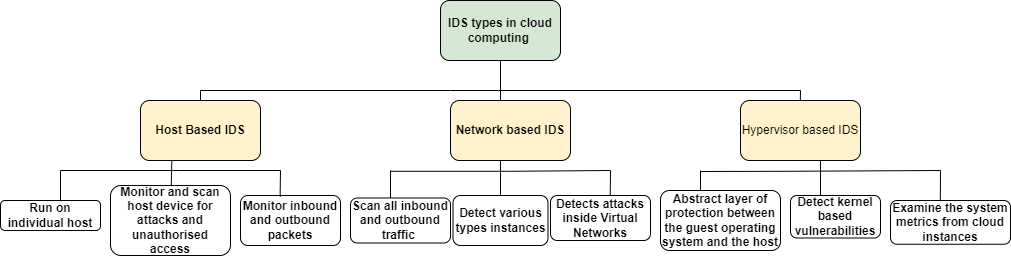
\includegraphics[width=1\linewidth]{ids.png}
		\caption{ three types of IDS that can be combined or separately used in cloud computing. Systems.\cite{mikail_2019_securing}}
		\label{fig:Ids}
	\end{figure}
	
	
	
	
	In Figure \ref{fig:Ids}, the diagram conveys that in a secure large environment, a network may comprise many IDS to prevent a majority of threats. One may prefer to have many IDS deployed to have a secure environment and therefore pointing to a very important note; solely deploying a network-based IDS cannot guarantee a near-to-secure environment.
	
	Various industry standard implementations of IDS are available for use in large network infrastructures. However, in this project, only threats captured by Suricata are studied for this project. As Security Onion is using a state-of-the-art intrusion detection technique by leveraging Suricata, the performance and accuracy of the system are proven to be high under a high network load \cite{mikail_2019_securing}.
	
	
	Numerous methods have been suggested in the literature to implement Security Onion for different purposes. However, this project will focus solely on implementing them in a general simulated network and leave the flexibility to be extended further for a specific use case.
	
	
	According to Hindy et al., the most common type of threats are Denial Of Service (DoS) and Distributed  Denial Of Service(DDoS), this is whereby a malicious user occupies the network by flooding it with resources, causing the system to become unresponsive, an example of this daily would be a big event or breaking news \cite{hindy_2020_taxonomy}. Dos and DDoS can fall into the following categories:
	
	\begin{itemize}
		\item Flood Attack - refers to flooding the system with high volumes of requests exhausting the system's bandwidth making the network unavailable for other users to use \cite{sonar_2014_survey}.
		\item Amplification Attack - also known as Network Time Protocol (NTP) amplification attack, causes the network to become unavailable through the use of one or more compromised applications sending more UDP traffic than the targeted network can handle \cite{sonar_2014_survey}. 
		\item Protocol Exploit - is whereby an attacker alters internal content by bugging the network's protocol to exhaust the operating system's resources \cite{sonar_2014_survey}.
		\item Malformed Packets - causes the network service to be overloaded with packets that may seem clean from threats, but indeed are malformed, bugged to fail the service \cite{alenezi_2012_methodologies}.
	\end{itemize}
	
	
	
	
	Several other attacks are in common with the public cloud in terms of network threats that impact users' data and the integrity of the organisation. These attacks include:
	\\
	
	\begin{itemize}\label{ICMP}
		\item \textbf{Smurf Attack} also known as an ICMP DoS is an example of a Reflection-Based flooding attack, in which the attacker creates a fake echo containing the target IP addresses which is then broadcasted to all hosts in that network. The hosts then reply to the broadcast accumulating into volumes of Internet Control Message Protocol (ICMP) packets making the network inoperable. ICMP is used by routers to test the reachability of a destination \cite{kumar_2007_smurf}.
		\begin{center}
			\begin{figure}[H]
				\centering
				\includegraphics[width=0.8\linewidth]{smurf attack.png}
				\caption{Smurf attack's Infrastructure \cite{kumar_2007_smurf}}
				\label{fig:Smurf}
			\end{figure}
		\end{center}
		
		
		
		
		\begin{lstlisting} [escapeinside={(*}{*)}, numbers=right]
			hping3 ####.####.####.####-q -ICMP -C 3 -K 4 (*\textcolor{red}{\footnote{this was extracted from a thesis on Testing the Security Onion by Kayla Jansen. \cite{jansen_2018_testing}}}*) \end{lstlisting} 
		In this command, the hashes represent the IP address of the victim and must be swapped for the hashes \cite{jansen_2018_testing}.
		
		
		
		
		\item \textbf{SYN flood} This type of attack occurs by looking for a known vulnerability in the Transmission Control Protocol (TCP) connection which validates authentication using a sequence of communication. The sequence is initiated when the client sends a SYN message to the server, the server then replies with the SYN message and attaches its message. If the client can decrypt the message and send it back to the server with the attached encrypted message (in this case "ACK"), the authentication is deemed successful. 
		\\
		An SYN attack occurs when an attacker floods the server with multiple SYN requests, the server in turn, replies and waits for the client to respond this uses up the resource while preventing the target network to be accessed.
		
		\begin{center}
			\begin{figure}[H]
				\centering
				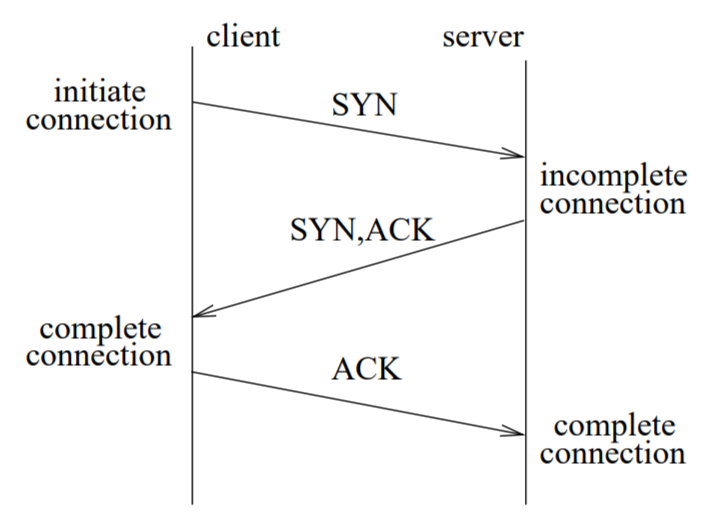
\includegraphics[width=0.45\linewidth]{ syn.png}
				\caption{SYN flood's Infrastructure \cite{lemon_2002_resisting}}
				\label{fig:syn}
			\end{figure}
		\end{center}
		In this project, this attack can be implemented by setting up Kali Linux and using the following command: \cite{jansen_2018_testing}
		
		
		\begin{lstlisting} [escapeinside={(*}{*)}, numbers=right]
			hping3 ####.####.####.#### -q -n -d 90 -S -p xx --flood -rand-source (*\textcolor{red}{\footnote{this was extracted from a thesis on Testing the Security Onion by Kayla Jansen. \cite{jansen_2018_testing}}}*) \end{lstlisting} 
		
		
		
		To implement this command successfully the IP address of the victim must be swapped for the hashes, then -d 90 can be changed to the size of packets the attacker would like to send, and the x needs to be changed for the port number \cite{jansen_2018_testing}.
		
		
		\item \textbf{UDP Flood } \label{UDP}this is a User Datagram Protocol (UDP)  whereby the attacker issues an attack on the Master Control Program (MCP) upon receiving the relevant information the MCP issues instructions to compromised systems to mask themselves using different IP addresses and repeatedly sending UDP packets directing to a random port. This causes the system to listen to the port, causing the system to wait for a response while more UDP packets are sent, eventually, this causes the system to crash. The figure \ref{fig:UDP} below is an illustration made to understand this concept better.
		
		
		\begin{center}
			\begin{figure}[H]
				\centering
				\includegraphics[width=0.75\linewidth]{ UDP.png}
				\caption{UDP flood's Infrastructure \cite{singh_2010_agent}}
				\label{fig:UDP}
			\end{figure}
		\end{center}
		
		To carry out a similar attack on Security Onion the following command comes in to use:	\begin{lstlisting} [escapeinside={(*}{*)}, numbers=right]
			sudo hping3 --flood -a \#.\#.\#.\# -2 -p x \#.\#.\#.\# (*\textcolor{red}{\footnote{this was extracted from a thesis on Testing the Security Onion by Kayla Jansen \cite{jansen_2018_testing}. }}*) \end{lstlisting} 
		As mentioned before the hashes represent IP addresses, the first set of hashes is the IP address the attacker masks themselves as. The last set of hashes the victim's IP addresses, x represents the port the victim's system is going to listen to.
		
		\textbf{Other types of attack include:}
		\item \textbf{The ping of Death} is another type of attack that occurs when the size of the packet attached to the ping sent exceeds 65,535 bytes which are significantly large for an Internet Protocol Version 4 (IPv4) router to process, therefore causing the packet to split. Attempting to reassemble the packets causes the system to overflow and the system goes into DoS \cite{sonar_2014_survey}.
		
		
		\item \textbf{XSS} also known as Cross-Site Scripting is an attack that occurs around sending a bugged client-side web application to a user. The attacker initially alters the website by injecting a bad script and defacing it or redirecting the user to a fake website. The attacker takes advantage of this by having access to sensitive data such as cookies.
		
		\item \textbf{Packet forging} also known as an injection is another type of attack where the packets sent can perform malicious activities such as accessing sensitive information \cite{hindy_2020_taxonomy}.
		
		
		\item \textbf{IP Spoofing} is used to gain unauthorized access, firstly the attackers must mask themselves by using a credible IP address that the target IP recognises as credible and trusts, the attacker would then disable the trusted IP's ability to access the network resources to prevent any unwanted intervention, the authentication process would then start, if successful, the attacker may now able to send a packet that has been tampered to have access in the future \cite{babu_2010_comprehensive}.
		
		
		\item \textbf{DNS spoofing} In this network threat the attacker redirects the user by inserting or altering the IP address to what seems like a legitimate website or server that is under the attacker's control.
		The following is a sequence in a normal scenario:
		\begin{itemize}
			\item The user sends a query to the DNS server.
			\item The DNS server replies to the user with the IP address.
			\item The user then connects to the IP address given by the server; redirecting them to the destination the user initially made a query on.
		\end{itemize}
		
		The following is a sequence of scenarios where an attacker is involved:
		\begin{itemize}
			\item The attacker identifies the server used by the user and tampers the IP address of a query to an IP the attacker can control without seeming suspicious.
			\item The user sends a query to the DNS server.
			
			\item The DNS server replies to the user with the IP address modified by the attacker.
			
			\item The user then connects to the IP address given by the attacker masked as the server; redirecting them to a fake page \cite{babu_2010_comprehensive}.	 
		\end{itemize}
		
		
		
		
		
		\item  \textbf{ARP spoofing (ARP poisoning)} ARP refers to Address Resolution Protocol, the attacker may use spoofing tools such as Parasiten, Ettercap, or ARPoison to look for a MAC and IP address to send a tampered ARP request to convince the target network to reply allowing the tools mentioned above to tamper, redirect another type of attacks such intercepting communication channels. 
		
		\item \textbf{Cloning} is an attack commonly used by attackers to impersonate a user to gain information \cite{hindy_2020_taxonomy}, there are real cases such as the NATO'S senior commander Admiral Jones identity being cloned, this was done to gain private information on government officials receiving and accepting  Facebook friendship requests from a cloned profile of Admiral Jones \cite{fire_2014_online}.
	\end{itemize}
	
	Common consensus by other researchers suggests that Security Onion is an off-the-shelf framework that provides detection and prevention of attacks on public and private clouds, as well as the simulated network this project will use.
	
	This report will aim to explore these attacks and implement Security Onion to detect and prevent these attacks in the project.
	
	
		
		
		
		\subsection{Different implementation of Network Intrusion Detection systems }
		
		Network Intrusion System (NIDS) refers to tools implemented in a framework to prevent incoming threats in a network to alter internal settings or retrieve personal information. NIDS is especially important due to the rise in cybercrime and the surging demand for a larger bandwidth to process packets at a higher speed. There are several approaches in which way users or large organisations decide to protect their environment.
		In this report NIDS' will be analysed and compared; this is done to extract information on how each infrastructure processes packets and how they single malicious packets.
		
		Due to the rampantly increased rates in cybercrime, it has become significantly difficult to process vast amounts of network packets using IDS such as Snort due to single threading, single threading can be exemplified by Figure \ref{fig:Snort} below; a diagram representing Snort's infrastructure originally published by (Gómez et al., 2009)\cite{gmez_2009_design}.
		\subsubsection{Snort}
		\begin{center}
			\begin{figure}[H]
				\centering
				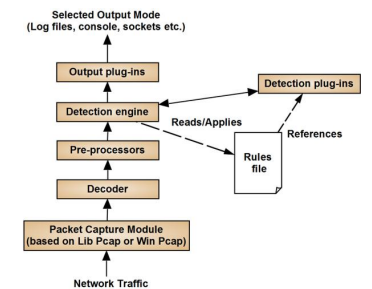
\includegraphics[width=0.6\linewidth]{snort.png}
				\caption{Snort's Infrastructure \cite{fekolkin_2015_intrusion}}
				\label{fig:Snort}
			\end{figure}
		\end{center}
		
		Initially, starting from the bottom of the infrastructure, network traffic, in essence, the packets, are fed into a network capture module, whereby an external library such as Lib Pcap is used as required by Snort to sniff packets, the decoder then processes these raw packets through a sequence of decoders each designated to decode specific components of the protocol such as their settings, packet size, and other hidden abnormalities. In the case a suspicious packet is detected, the decoder would then generate an alert \cite{fekolkin_2015_intrusion}. Next, the purpose of a pre-processor is to improve overall performance by preventing any form of rouge data from going into the next level, in essence, the preprocessor must ensure it combs through the traffic of data before sending it to the detection engine.
		To ensure this process is successful, the preprocessors must be configured appropriately. As further explained in the book Snort Intrusion Detection and Prevention Toolkit published by Beale, Baker, and Esler, many types of preprocessors can perform useful activities before packets reach the detection engine also known as the rule engine \cite{beale_2007_snort}, the table below is a few commonly known preprocessor names and their function: 
		
		\begin{center}
			\setlength{\tabcolsep}{10pt} % Default value: 6pt
			\renewcommand{\arraystretch}{1.5} % Default value: 1
			\begin{tabular}{ | m{3cm} | m{12cm}|  } 
				\hline
				Preprocessor & Function  \\ 
				
				\hline
				Frag3 & This preprocessor consists of a module that can handle fragmentation-based attacks on a user-specified target by reassembling IP fragments. It uses the target's TCP/IP stack to model its fragmentation behaviour. This preprocessor follows two steps 
				
				\begin{itemize}
					\item Global initialization phase
					\item Definition of defragmentation engines
				\end{itemize}
				
				This preprocessor is useful due to its extensive abilities, for instance, it may be required to apply specific policies to certain IP groups whilst having a default policy for all other traffic, this preprocessor can be configured to run multiple engines at the same time.
				%https://www.sciencedirect.com/topics/computer-science/preprocessors
				
				\\ 
				\hline
				Stream4 & This preprocessor is constructed of two modules:
				\begin{itemize}
					\item  Stateful analysis is a module that is used for detecting TCP state issues and port scans, and it requires careful configuration to optimize its performance
					\item Stream reassembly is known to perform complete stream reassembly for TCP and can manage both client and server streams, with options for specifying which ports to perform reassembly on and other directives.
				\end{itemize}
				
				\\ 
				\hline
				sfPortscan & A preprocessor designed that can detect scan techniques, it allows users to specify which protocols to monitor the type of scan and sensitivity level.
				To assign the flow of direction to connectionless protocols like UDP and ICMP flow processor can be used with these preprocessors, to avoid generating multiple alerts for the same scan packets it is recommended to disable evasion alerts in the stream4 preprocessor.\\ 
				\hline
			\end{tabular}
		\end{center}
		
		
		Going into the  detection engine, a set of predefined rules are applied to the incoming data, these rules are specially structured to analyse these packets for:
		
		\begin{itemize}
			
			\item A known signature of the attack to be detected \cite{gmez_2009_design}.
			\item The detection plug-ins permit the configuration of the engine \cite{gmez_2009_design}.
		\end{itemize}
		
		The output plug-ins would clarify where and how different types of alerts should be logged.
		Suricata is considered to be a more computationally advanced NIDS as its ability to overcome the limitations of single threading NIDS  surpasses the current concerns with the demand of larger bandwidth by processing large amounts of packets while maintaining a good speed; this is done through a process called multithreading whereas Snort would ignore packets that it gets flooded by due to not receiving enough bandwidth \cite{park_2016_performance}, Suricatas infrastructure on how it deals with managing multiple packets in the same environment is displayed in Figure \ref{fig:suricata}, handling many packets at the same time, has become especially important with malicious penetration methods constantly evolving and the necessity of having a rigorous process to ensure a secure environment is at hand.
		
		\subsubsection{Suricata}
		\begin{center}
			\begin{figure}[H]
				\centering
				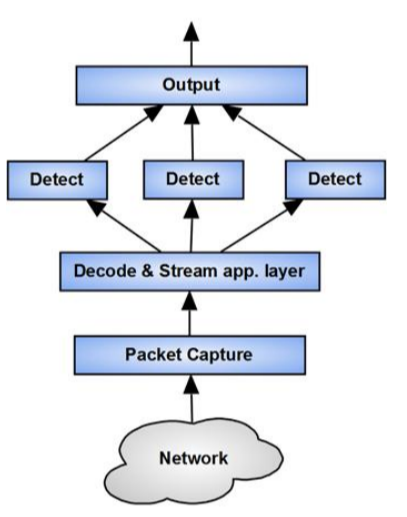
\includegraphics[width=0.5\linewidth]{suricata.png}
				\caption{Suricata's Infrastructure \cite{fekolkin_2015_intrusion}}
				\label{fig:suricata}
			\end{figure}
		\end{center}
		
		
		To begin, the traffic goes into the Packet capture to process the packets for analysis, then, just like Snort the packets go into the decoding layer with an additional feature called the stream app layer which essentially is a reassembly engine, this helps to assemble packets from incoming traffic to be sorted in a form of queue ready to go into the thread engine. Before going into the next layer, here, a Queue Handler function is invoked where packets are either being fetched into a thread or ditched, going through this layer consists of multiple threads detectors that fetch packets from the thread and detect malicious threats by putting the signature against a database consisting predefined set of signatures known to be threats to base the decision whether the packet can enter the network or be dropped \cite{fekolkin_2015_intrusion}.
		
		
		
		
		
		\subsection{ Analysing Network Simulation}		
		
		
		To execute the implementation of this project, a network topology must be first designed and analysed for faults or further adjustments, doing so may allow a more successful deployment. 
		
		Simulations are considered a necessity to help in the process of building new technologies as this gives developers an idea of what is to be expected had their prototype has been developed in a real environment at a larger scale where the impact is real. A network simulator refers to an interactive software tool that allows network designers/engineers to design a topology at a smaller case with little to no impact, this allows designers to observe and calculate the network's behaviour ensuring it is suitable for real-life implementation. Implementing a network in a real environment can be very difficult and costly, thus observing how a network behaves in a simulated environment when a new protocol is implemented may aid the process of ensuring the network's topology is safe to deploy in a real environment with little to no errors which are important to prevent accidents to occur.
		
		
		
		\begin{center}
			\begin{figure}[H]
				\centering
				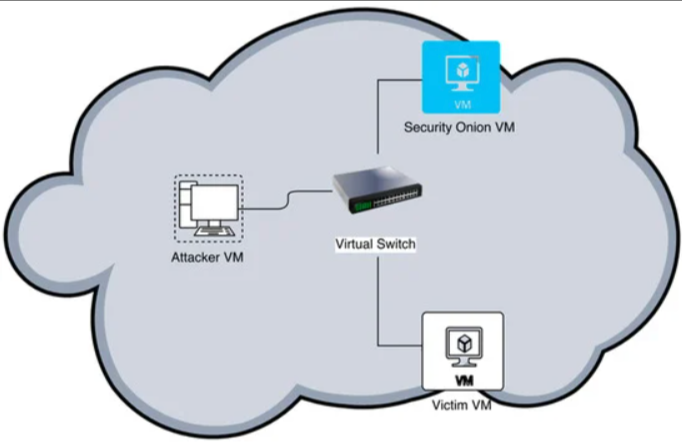
\includegraphics[width=0.5\linewidth]{topology1.png}
				\caption{Network Topology  \cite{mikail_2019_securing}}
				\label{fig:topology1}
			\end{figure}
		\end{center}
		The experiment carried out by Mikail and Pranggono revolved around Snort and testing the security of cloud computing.
		To experiment with integrated tools  Security Onion comes with, Figure \ref{fig:topology1} used by Mikail and Pranggono, which revolves around three VMs:
		\begin{itemize}
			\item Security Onion generates alerts through the intrusion detection system.
			\item Kali Linux acts as the attacker's system.
			\item Metasploitable acts as the victim's system.
		\end{itemize}
		All three VMs in this configuration are connected through a switch. 
		Although Figure \ref{fig:topology1} is a single realistic configuration, a concern this project can alter is releasing more than one attack. Back to this project, in this experiment one NIDS is being tested whose results will be then put against existing results.
		
		\begin{center}
			\begin{figure}[H]
				\centering
				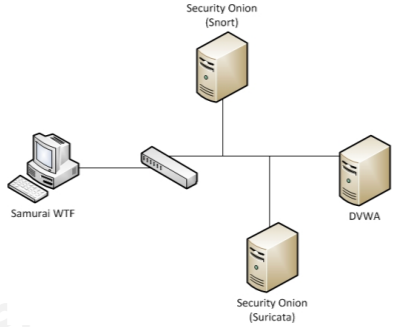
\includegraphics[width=0.5\linewidth]{topology2.png}
				\caption{Network Topology \cite{deuble_2012_detecting}}
				\label{fig:topology2}
			\end{figure}
		\end{center}
		Another network simulation experiment executed by Deuble, A. Security involved testing both Suricata and Snort on detecting web application-based attacks. the topology  is similar to the previous Figure \ref{fig:topology2}; however this topology consist of four components:  \cite{deuble_2012_detecting}
		
		
		
		\begin{itemize}
			\item Security Onion alerts and prevents intrusion detection using Suricata.
			\item Security Onion alerts and prevents intrusion detection using Snort.
			\item Samurai distribution acts as the attacker's system.
			\item Damn Vulnerable Web Application acts as the victim's system.
		\end{itemize}
		All 4 VMs in this configuration are connected through a switch. 
		In this Figure \ref{fig:topology2} all four components are interconnected, and the topology gives more accurate results as both Snort and Suricata generate alerts upon detection. 
		
		
		
		
		\begin{center}
			\begin{figure}[H]
				\centering
				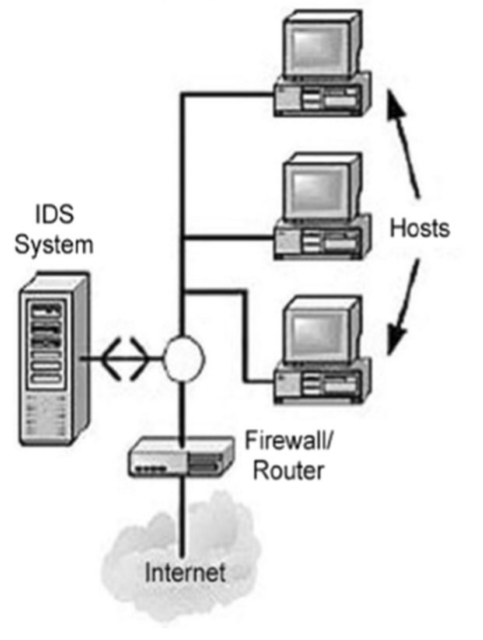
\includegraphics[width=0.3\linewidth]{topology3.png}
				\caption{Network Topology \cite{park_2016_performance}}
				\label{fig:topology3}
			\end{figure}
		\end{center}
		One last example of topology is in Figure \ref{fig:topology3} where there is no experiment involved. Although this is what typical settings look like it is not applicable as in this project a controlled environment is required to send threats that can be damaging to the system.
		
		
		\section{Methodology}\label{1}
		%\textbf{INCLUDE FINDINGS AND THEIR CONCLUSIONS LOGICAL TRANSITIONS}
		An ample amount of research has been done to find an IDS that is the most fitting to cover all ranges of threats and all sizes of packets, Suricata is one of many NIDS that is considered early in its life cycle and has a few scholarly activities but not many extensive documentations were found, this might convey why there is a lack of organisation and day to users implementing this NIDS in their system. 
		This section of the literature review covers the research done on different NIDS, methodologies findings conclusions based on the findings.
		
		One evident difference pointed out in the article by Fekolkin mentions a key factor that differentiates Suricata and Snort methods of threading packets, Snort was designed to run on single-core processors, this can become costly in the future and disadvantageous to users who value performance, and as the network grows. However, Snort can be seen progressing to tackle these issues in the near future, through a fairly new Hybrid IDS called H-Snort which is a redesign of the preprocessor to essentially detect anomalies and many more extensive features \cite{gmez_2009_design}. On the other hand, Suricata's multithreading engine makes use of the computational power by having multi-core processing units allowing more efficiency in processing multiple large packets while maintaining speed, the opportunity to have a scalable IDS as users can configure the number of thread detectors to run in the same environment can be advantageous from a financial perspective \cite{fekolkin_2015_intrusion}.
		
		An article published by Albin and Rowe carried out a comparison experiment between the two NIDS by sending threats in a controlled environment. Albin measured detection performance and accuracy in an active virtual environment by measuring the following:
		\begin{itemize}
			\item CPU percentage. 
			\item Memory usage.
			\item Network usage.
		\end{itemize}
		To further note, the network tap had been used to compare the two NIDS  had a network bandwidth of 20 Gbps which is a considerably large pipe where traffic has an average of 200Mbps \cite{albin_2012_a}, the signatures came from two IDS rule maintainers, SourceFire Vulnerability Research Team (VRT) and Emerging Threats (ET).
		In total three experiments were carried out.
		Experiment one was carried out to compare the monitoring of the traffic, Albin noted the results conveyed that although Suricata used more computational resources Suricata still managed to use less CPU (50-60\% range) than Snort (60-70\% range), suggesting implementing Suricata might not have 
		
		
		In the first experiment, Albin et al. also noted that Suricata is "more memory-intensive", the memory usage started from 1.5 GB to 3.3Gb whereas for Snort it seems to be a bit more consistent from 0.8Gb to 1Gb \cite{albin_2012_a}. Below are two side-by-side Figures \ref{fig:ram} Suricata and Snort representing RAM usage:
		
		\begin{center}
			\begin{figure}[H]
				\centering
				\subfloat[\centering Suricata]{{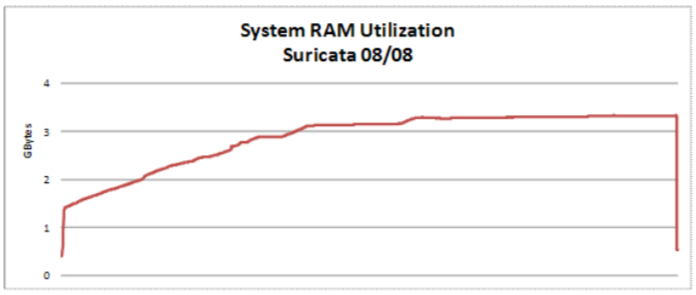
\includegraphics[width=0.4\linewidth]{suricata1.png} }}%
				\qquad
				\subfloat[\centering Snort]{{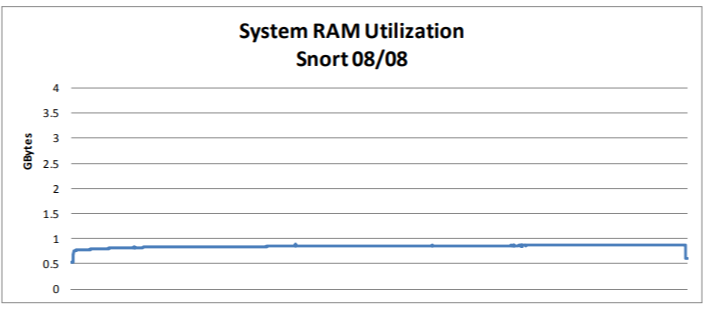
\includegraphics[width=0.4\linewidth]{snort1.png} }}%
				\caption{RAM usage by the two NIDS \cite{albin_2012_a}}%
				\label{fig:ram}%
			\end{figure}
		\end{center}
		
		
		Continuing, due to technical issues although the network traffic rate could not be recorded, the averages are in the Figures \ref{fig:rate} below.
		
		\begin{center}
			\begin{figure}[H]
				\centering
				\subfloat[\centering Suricata 33,731/s packets]{{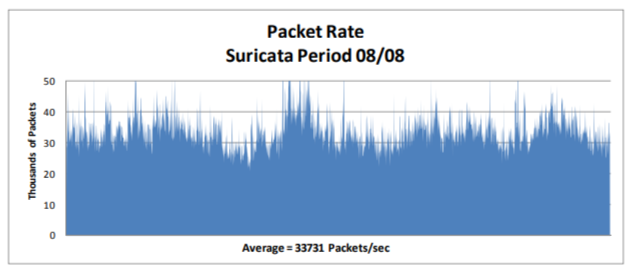
\includegraphics[width=0.4\linewidth]{suricata2.png} }}%
				\qquad
				\subfloat[\centering 20,090/s packets]{{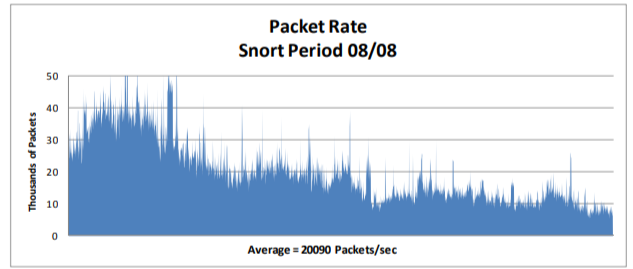
\includegraphics[width=0.4\linewidth]{snort2.png} }}%
				\caption{Network packets processed per second \cite{albin_2012_a}}%
				\label{fig:rate}
			\end{figure}
			
			
			
		\end{center}
		Given the findings, a similar methodology to this section will be used as a guide when evaluating the findings of this project.
		
		%White, J. S., Fitzsimmons, T., & Matthews, J. N. (2013, May).
		%Quantitative analysis of intrusion detection systems: Snort and
		%Suricata. In SPIE Defense, Security, and Sensing (pp. 875
		
		
		
		
		
		
		
		
		
		\section{Analysis and Design
		}
		
		From this section onwards the report will be a record of the transition from research to implementation.
		
		\subsection{Designing The Network Topology}
		The figure below is a diagram that has been designed for this project:
		
		
		\begin{center}
			\begin{figure}[H]
				\centering
				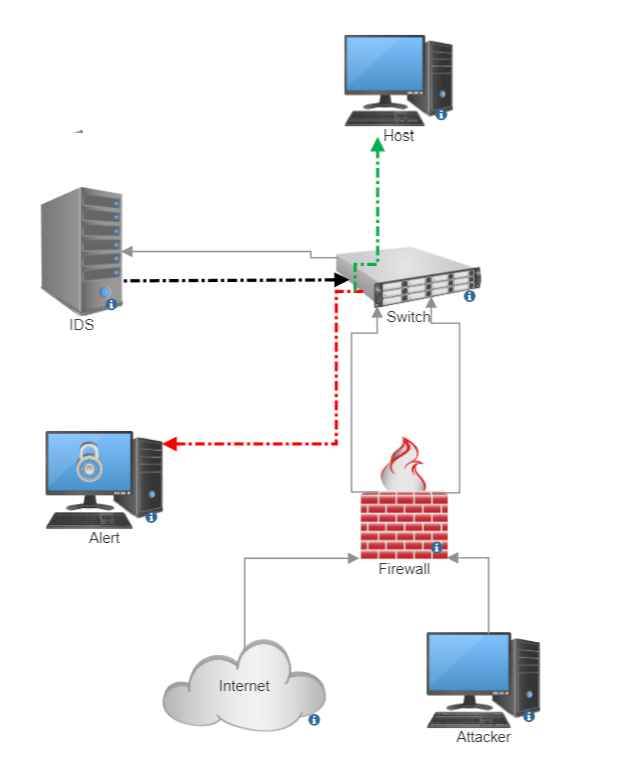
\includegraphics[width=0.5\linewidth]{design.png}
				\caption{A design of this project's topology} 
				\label{fig:design}
			\end{figure}
		\end{center}
		
		The topology mapped in figure \ref{fig:design} displays how this project is going to set the environment for network threats in the Security onion, an attacker is required to ensure safety is not compromised, and the threats would travel from the source IP address of the Kali Linux environment to the target address on the Security Onions environment. The attacker's device Kali in this case, can for instance flood the host's device with pings, overflowing the system enough to create a DOS attack, this would be detected by the Intrusion Detection System (IDS) which would be flag alerts on the dashboard and log it into the system to be viewed. One thing to be noted in this project is that a different route has been taken than what has been proposed in the proposal. Security Onion as a proxy in-between the network and the outside network layer in a simulated network is longer being implemented as it's not as realistic as it would be if real virtual environments are used.
		\subsection{Data Collection}
		To have a look at the alert system, as mentioned previously the user would be required to access the Security Onion's dashboard, testing around the filters and adding tools gives a good understanding of each threat that is sent, for instance, in an attack where the IP source IP is not specified, the user would need to expand on the unspecified attack the user can access the dashboard to this  \href{https://10.0.2.0/kibana/app/dashboards#/view/30d0ac90-729f-11ea-8dd2-9d8795a1200b?_g=(filters:!(),refreshInterval:(pause:!t,value:0),time:(from:now-24h,mode:quick,to:now))}{link} which is a good site to start with for users with all the necessary filters they should look for when testing attacks. As expected in the table there's no IP address pointing to where this threat is coming from. In this case, adding in the following column would be required.
		\begin{center}
			\begin{figure}[H]
				\centering
				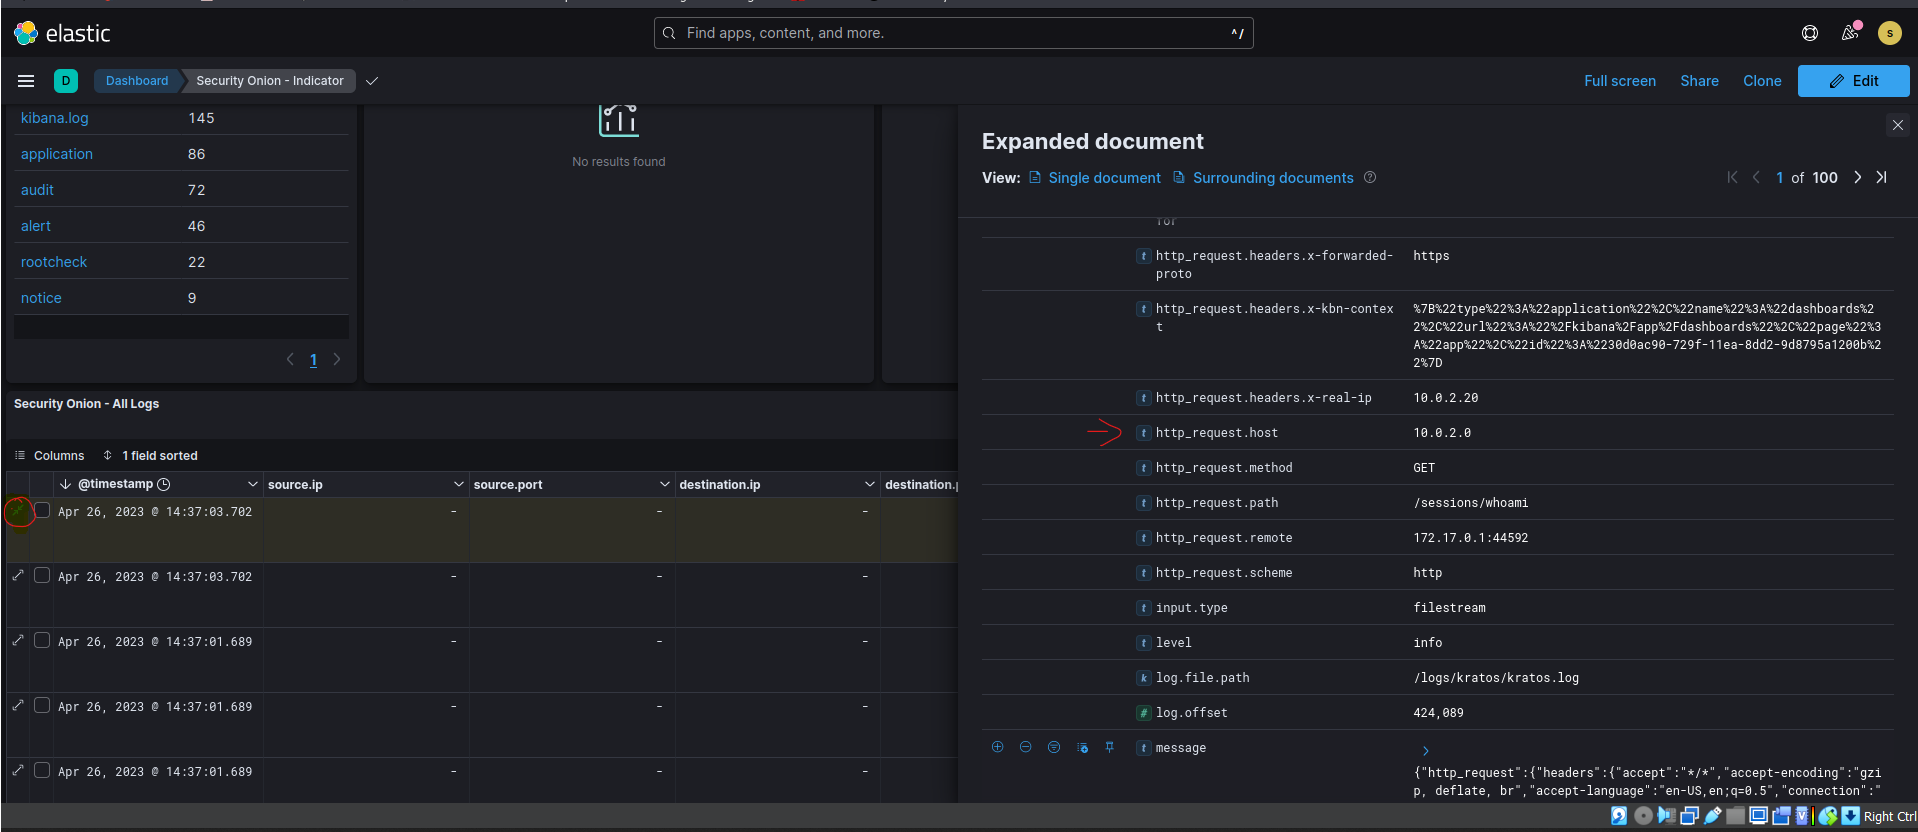
\includegraphics[width=1\linewidth]{link.png}
				\caption{Security Logs from the SO's dashboard. } 
				\label{fig:18}
			\end{figure}
		\end{center}
		
		This data can further be accessed in JSON format under "message", in the case the user would like more detail in a compact version. The flooding threats to be sent will be sent for about 45 seconds.
		
		Overall implementing the architecture in \ref{fig:design} has been a straightforward task due to decision to design the topology first. Because of this, it is much more convenient to collect data in this way.
		
		\section{Implementation
		}
		\subsection {Installing Security Onion and Kali Linux}
		To initiate the installing program a virtual box is required, this allows virtual machines to be installed. This section will cover the installation process of Kali and Security Onion.
		The basic configuration for Security Onion and Kali are as follows:
		
		\begin{center}
			\begin{figure}[H]
				\centering
				\subfloat[\centering Security Onion's settings \label{18a}]{{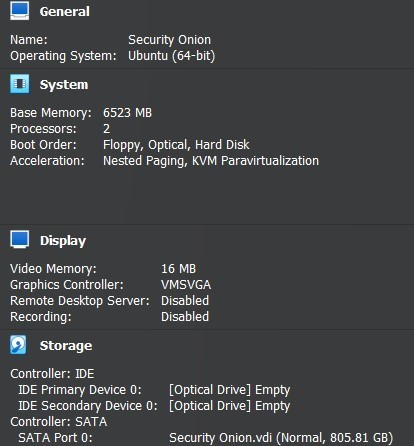
\includegraphics[width=0.44
						\linewidth]{start sec.jpg} }}%
				\qquad
				\subfloat[\centering Kali 's settings]{{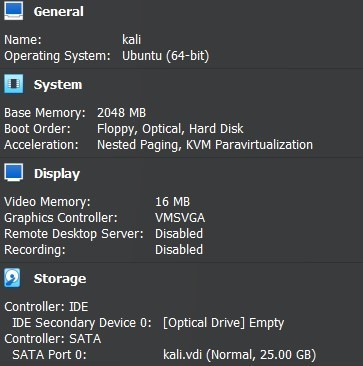
\includegraphics[width=0.45\linewidth]{start kali.jpg} }}%
				\caption{Network packets processed per second.}%
				\label{fig:install}
			\end{figure}
			
		\end{center}
		Before proceeding to start an optical disk with the drive of the machine installed should be added, the iso file can be downloaded from the documentation website. Although this can be done at the start of the configuration, it can also be added later by going to the setting, then storage then adding the file through the plus button of the controller IDE.
		
		To ensure the virtual machines can communicate in the settings under the network the following should be the configuration:
		
		\begin{center}
			\begin{figure}[H]
				\centering
				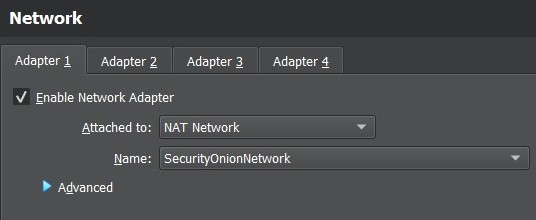
\includegraphics[width=0.5\linewidth]{start sec2.jpg}
				\caption{Network settings for both Security Onion and Kali  } 
				\label{fig:nat}
			\end{figure}
		\end{center}
		
		Starting with Security Onion a prompt message will appear requesting for a username and password.
		
		\begin{center}
			\begin{figure}[H]
				\centering
				\subfloat[\centering Username and password needs to be set]{{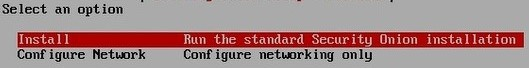
\includegraphics[width=0.45
						\linewidth]{3.jpg} }}%
				\qquad
				\subfloat[\centering Depending on the type of installation the setup will give different configuration outputs. ]{{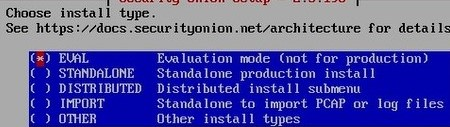
\includegraphics[width=0.45\linewidth]{4.jpg} }}%
				\caption{The beginning of the configuration for Security Onion.}
				\label{fig:Starting}
			\end{figure}
			
		\end{center}
		
		\begin{center}
			\begin{figure}[H]
				\centering
				\subfloat[\centering The hostname can be changed or left at the default name.]{{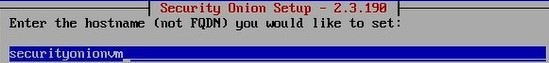
\includegraphics[width=0.45
						\linewidth]{7.jpg} }}%
				\qquad
				\subfloat[\centering Management NIC]{{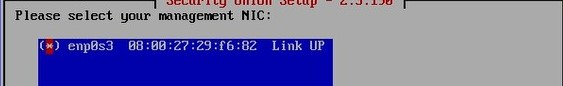
\includegraphics[width=0.45\linewidth]{8.jpg} }}%
				\caption{Configuring hostname and Management NIC }
				\label{fig:Starting}
			\end{figure}
			
		\end{center}
		
		\begin{center}
			\begin{figure}[H]
				\centering
				\subfloat[\centering In order to establish communications, IP was chosen]{{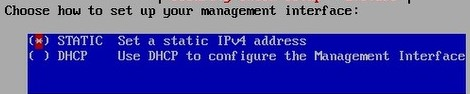
\includegraphics[width=0.45
						\linewidth]{9.jpg} }}%
				\qquad
				\subfloat[\centering Setting Security Onion's IP address]{{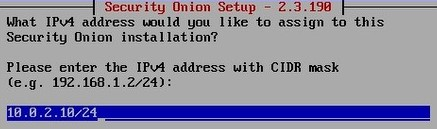
\includegraphics[width=0.45\linewidth]{10.jpg} }}%
				\caption{Setting up the network.}
				\label{fig:Starting}
			\end{figure}
			
		\end{center}
		
		
		
		\begin{center}
			\begin{figure}[H]
				\centering
				\subfloat[\centering Setting the gateway IP address]{{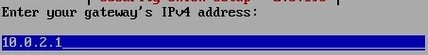
\includegraphics[width=0.45
						\linewidth]{11.jpg} }}%
				\qquad
				\subfloat[\centering The DNS server address has been kept to default.]{{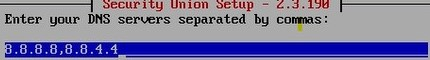
\includegraphics[width=0.45\linewidth]{12.jpg} }}%
				\caption{Setting SO's gateway IP and DNS server.}
				\label{fig:Starting}
			\end{figure}
			
		\end{center}
		
		
		\begin{center}
			\begin{figure}[H]
				\centering
				\subfloat[\centering  The DNS search domain is kept to default.]{{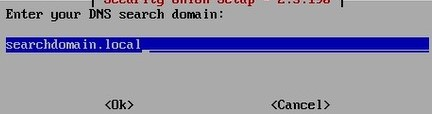
\includegraphics[width=0.45
						\linewidth]{13.jpg} }}%
				\qquad
				\subfloat[\centering Internet access is required in this project .]{{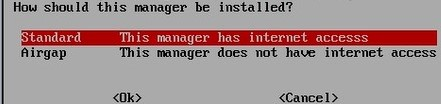
\includegraphics[width=0.45\linewidth]{15.jpg} }}%
				\caption{Setting up the DNS search domain and installing the manager.}
				\label{fig:Starting}
			\end{figure}
			
		\end{center}
		
		
		\begin{center}
			\begin{figure}[H]
				\centering
				\subfloat[\centering Username and password needs to be set]{{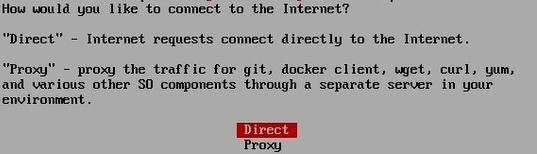
\includegraphics[width=0.45
						\linewidth]{16.jpg} }}%
				\qquad
				\subfloat[\centering Only one option was given as initially only one network adapter was configured; see Figure \ref{fig:nat}]{{
\includegraphics[width=0.45\linewidth]{17.jpg} }}%
				\caption{Configuring access to the internet and choosing NICs.}
				\label{fig:Starting}
			\end{figure}
			
		\end{center}
		
		\begin{center}
			\begin{figure}[H]
				\centering
				\subfloat[\centering This part is kept to default.]{{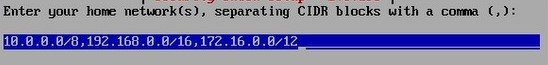
\includegraphics[width=0.45
						\linewidth]{19.jpg} }}%
				\qquad
				\subfloat[\centering The Virtual machine's communication will be established through configuring the IPs.]{{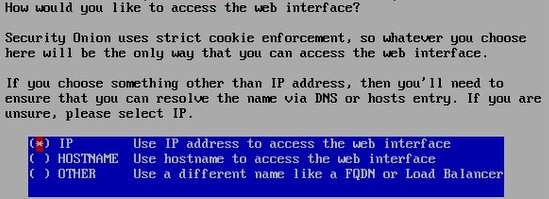
\includegraphics[width=0.45\linewidth]{23.jpg} }}%
				\caption{Setting up the network.}
				\label{fig:Starting}
			\end{figure}
			
		\end{center}
		
		\begin{center}
			\begin{figure}[H]
				\centering
				\subfloat[\centering Ntp needs to be configured therefore yes.]{{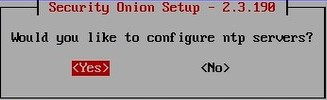
\includegraphics[width=0.45
						\linewidth]{24.jpg} }}%
				\qquad
				\subfloat[\centering The ntp server has been kept to default.]{{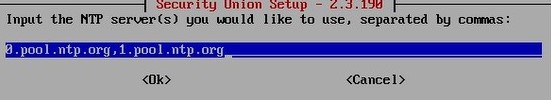
\includegraphics[width=0.45\linewidth]{25.jpg} }}%
				\caption{The beginning of the configuration for Security Onion.}
				\label{fig:Starting}
			\end{figure}
			
		\end{center}
		
		\begin{center}
			\begin{figure}[H]
				\centering
				\subfloat[\centering Another IP address later to be configured to the Kali  Virtual Machine's (VM) address]{{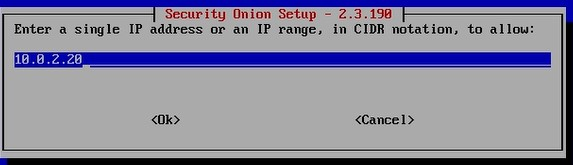
\includegraphics[width=0.45
						\linewidth]{27.jpg} }}%
				\qquad
				\subfloat[\centering A summary of the configuration.]{{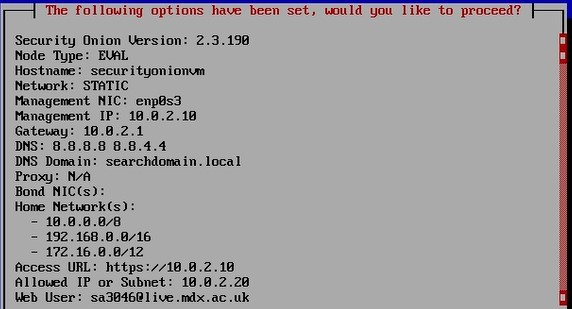
\includegraphics[width=0.45\linewidth]{28.jpg} }}%
				\caption{Setting an IP later to be Kali's VM and a summary of SO'S configuration}
				\label{fig:Starting}
			\end{figure}
			
		\end{center}
		
		
		\begin{center}
			\begin{figure}[H]
				\centering
				\subfloat[\centering All configurations have been left to default in Kali apart from the figure above]{{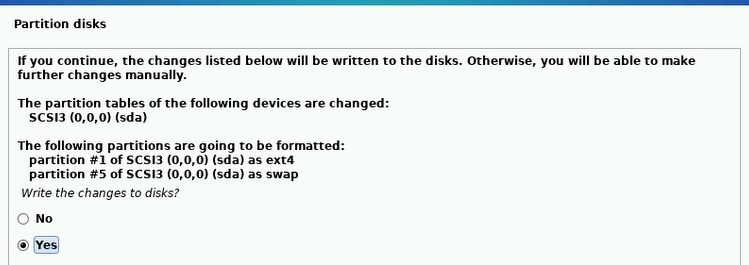
\includegraphics[width=0.45
						\linewidth]{38.jpg} }}%
				\qquad
				\subfloat[\centering An unsuccessful ping suggests there is no connection to the internet and Security Onion.]{{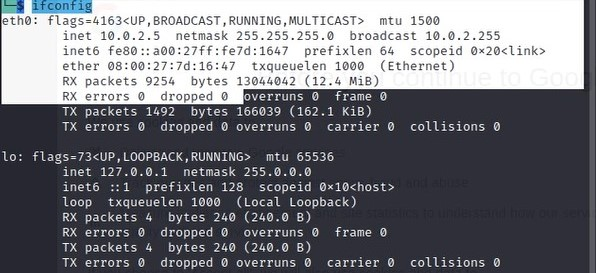
\includegraphics[width=0.45\linewidth]{40.jpg} }}%
				\caption{Configuring the Kali Linux machine and later pinging Security Onion. }
				\label{fig:Starting}
			\end{figure}
			
		\end{center}
		\subsection{Basic configuration}
		
		
		\begin{center}
		\begin{figure}[H]
			\centering
			\subfloat[\centering In the settings under network advanced configurations the Security Onion's IP address needs to be entered. ]{{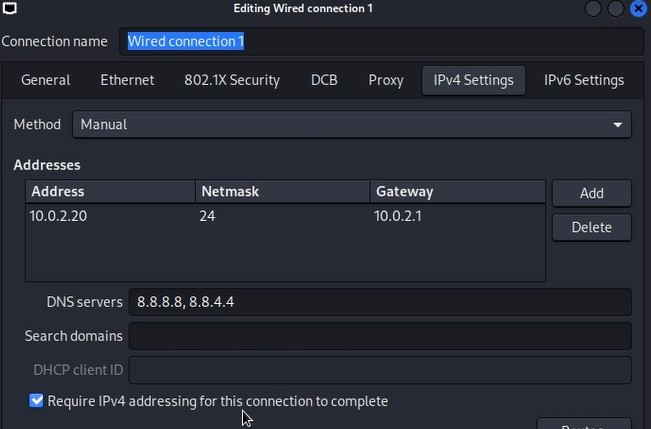
\includegraphics[width=0.45
					\linewidth]{42.jpg} }}%
			\qquad
			\subfloat[\centering If the ping is successful the configuration is also successful]{{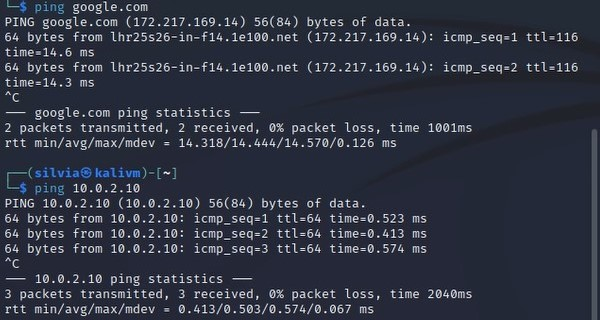
\includegraphics[width=0.45\linewidth]{43.jpg} }}%
			\caption{Configuring the Security Onion's IP address in Kali Linux}
			\label{fig:Starting}
		\end{figure}
		\end{center}
		\begin{center}
		\begin{figure}[H]
			\centering
			\subfloat[\centering Enter the IP Security Onion has been configured with.]{{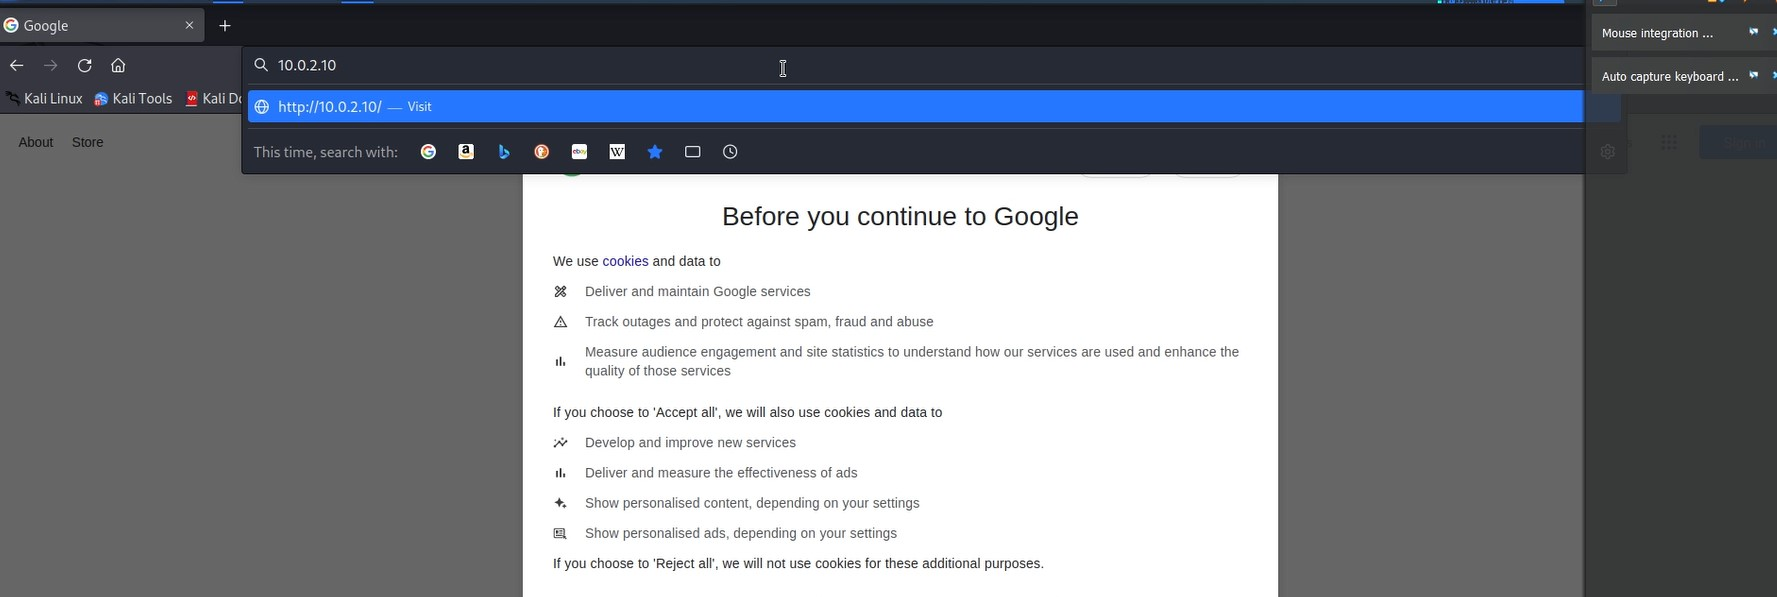
\includegraphics[width=0.45
					\linewidth]{45.jpg} }}%
			\qquad
			\subfloat[\centering Here the email address entered while configuring Security Onion must be entered to access the dashboard. \label{31b}]{{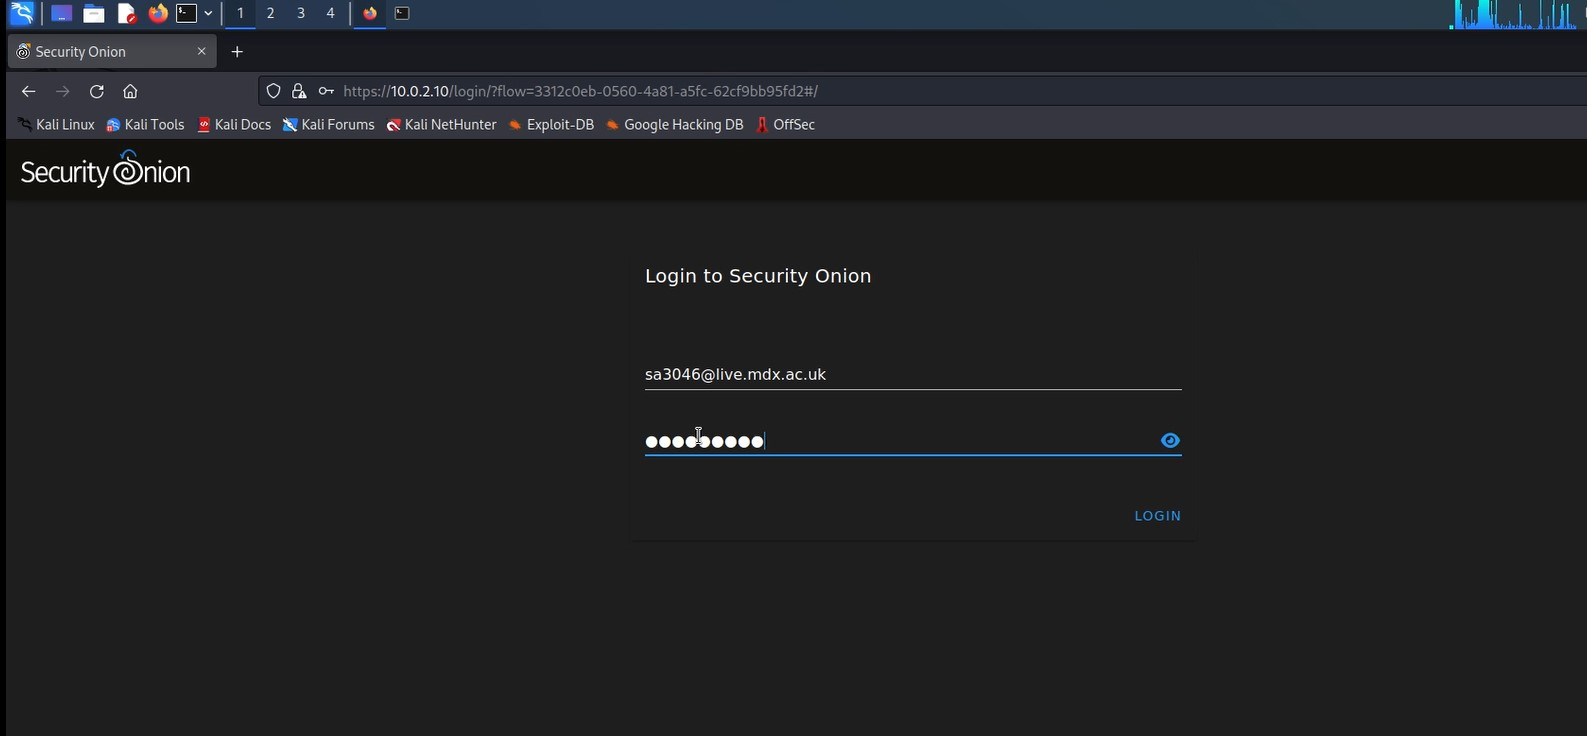
\includegraphics[width=0.45\linewidth]{46.jpg} }}%
			\caption{Accessing the Security Onion dashboard through Linux}
			\label{fig:pingtest}
		\end{figure}
		
		\end{center}
		
		\begin{center}
		\begin{figure}[H]
			\centering
			\subfloat[\centering The above displays dashboards and all the tools Security Onion comes in-built this may take a while to load. ]{{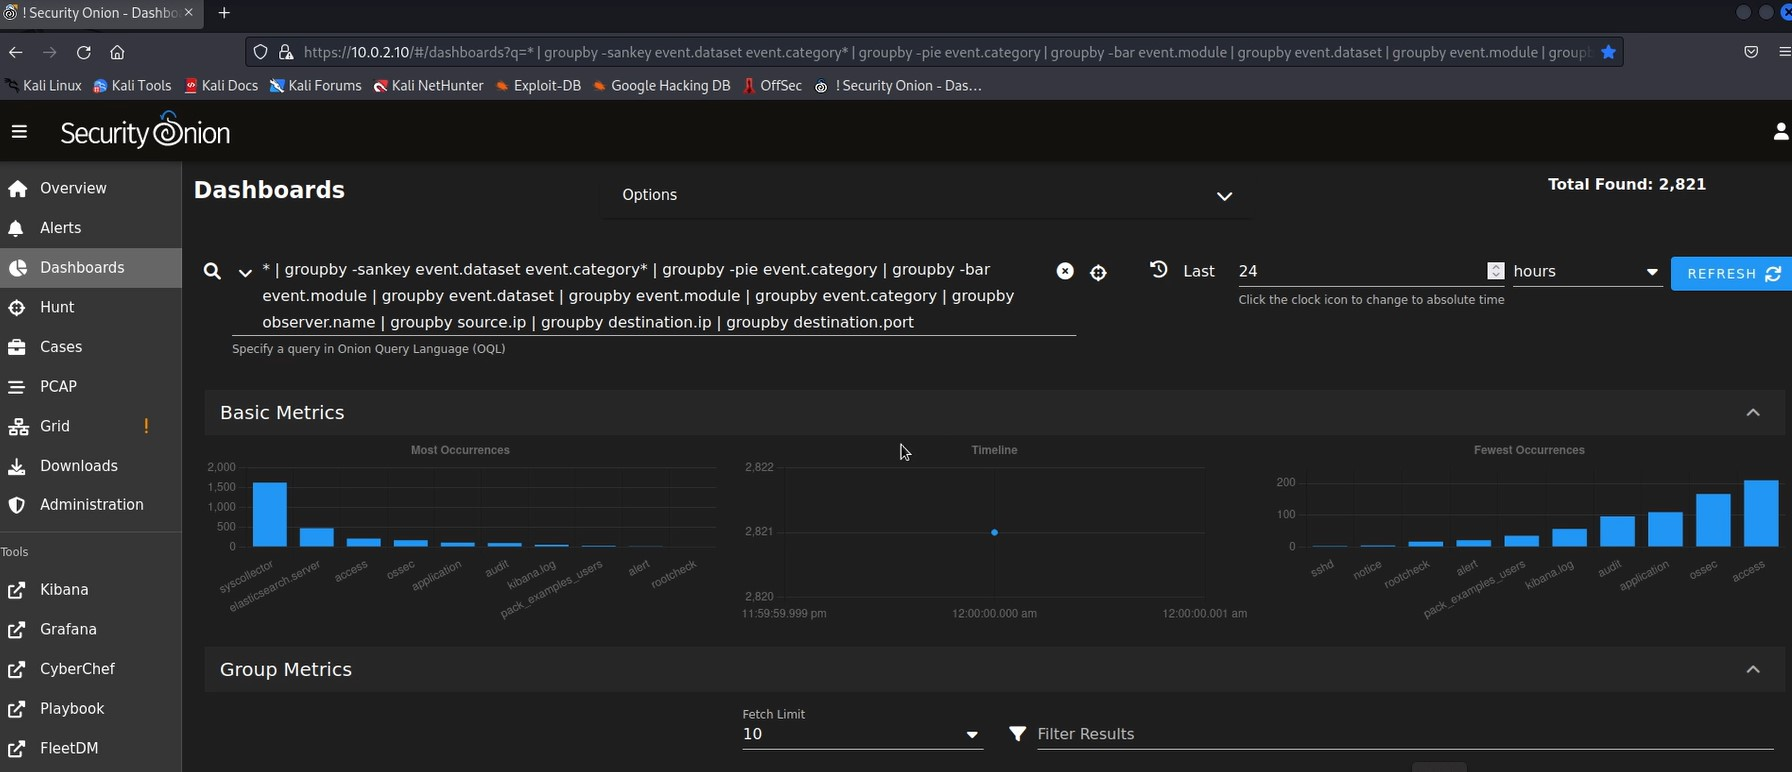
\includegraphics[width=0.45
					\linewidth]{49.jpg} }}%
			\qquad
			\subfloat[\centering With the command sudo so-status the status of each tool can be seen to make sure all tools can be accessed. \label{32b} ]{{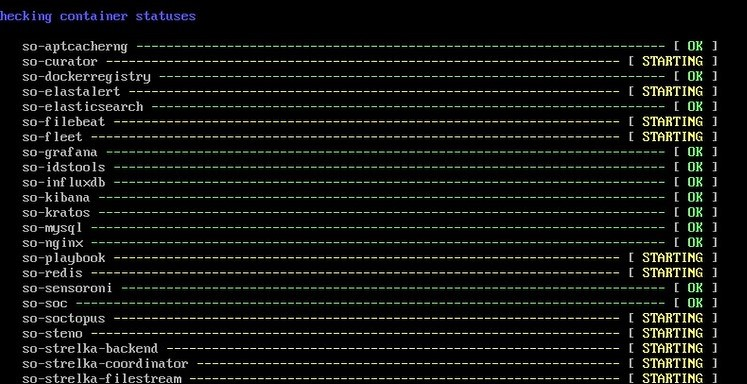
\includegraphics[width=0.45\linewidth]{48.jpg} }} 
			\caption{Display the dashboard and check the status of the tools.}
			\label{fig:Starting}
		\end{figure}
		
		\end{center}
		To ensure NIDS Suricata is working in the following directory:
		
		
		\begin{lstlisting}[language=bash]
		cd /etc/nsm/rules/local.rules
		\end{lstlisting}
		
		
		the following command is entered:
		\begin{lstlisting}  [language=bash]
		Alert icmp 10.1.1.1 any -> any (msg:"ICMP";
		sid:100002;)
		\end{lstlisting}
		
		
		
		To ensure a thorough experiment Suricata must be carried out in a controlled environment. This project aims to focus examine the overall performance of CPU, memory usage, and packet processing rates. 
		
		
		
		
		
		
		
		\section{Testing and Results} \label{testing}
		To ensure Kali can reach the target device a ping test should be done to ensure, Kali's attacks are being received in the first place.
		\begin{lstlisting}  [language=bash]
		ping 10.0.2.20
		ping google.com
		\end{lstlisting}
		The understanding behind a ping test is that an ICMP request is sent from the Kali virtual machine to check if a connection exists, if this is the case the Security Onion will echo a reply back. Figure \ref{32b} shows Kali has a connection established to both Security Onion and Google.com  
		
		
		\subsection{Sending attacks}
		
		
		Starting with Nmap Port-scanning, the purpose of this type of attack is to attain real-time information about the target IP address from whether the host is Up (or DOWN) to information on which ports are open at the current time, as it can be seen from the figure below this valuable information for a malicious user to send tailored attacks.
		
		\begin{lstlisting}  [language=bash]
		sudo nmap -sTU -sV -p x #.#.#.#
		\end{lstlisting}
		The format of this threat is as follows:
		To understand this low-level threat, "sudo" is necessary as root permission is required to run the command, moving on, the "nmap" command is used to scan whether the host is up and which ports are open for the IP provided. As for "-sTU" the s stands for scanning both "T" and "U" where "T" refers to the  TCP scan type. This is where Nmap will either do a TCP Sync scan or a TCP connect scan. The type of scan that will be done will be dependent on the user's privileges however by default it is usually a TCP SYN scan. The following switch -sV determines the service version running on that port. The -p refers to the x as the port numbers being scanned. And lastly, the \#'s represent the target IP addresses.
		
		
		
		\begin{center}
		\begin{figure}[H]
			\centering
			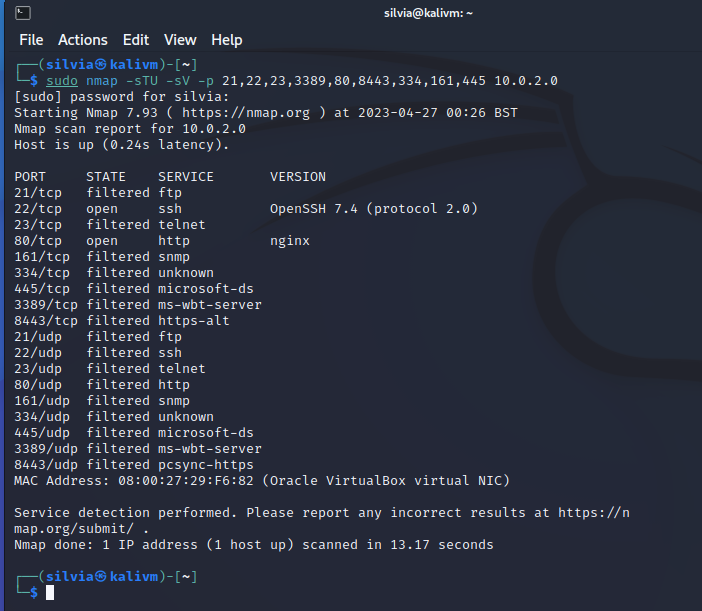
\includegraphics[width=1\linewidth]{portscanning.png}
			\caption{Portscanninng Security Onion take at 00:27. Results can be viewed in section \ref{attack1}} 
			\label{fig:29}
		\end{figure}
		\end{center}
		
		Figure \ref{fig:29} can be used to conclude that Kali's system was able to successfully establish communication with the target device. This is inferred from no error messages being displayed and that the host is up and is scanned in two ports through TCP (22/TCP and 80/tcp).
		
		To view the impact on the overall environment Grafana has been used. The guide to using Grafana will be given in the User Guide section. \ref{userguide}An important note be made here is that Nmap can be used for both ethical and malicious reasons, where one can use it to find vulnerabilities to prevent and protect within their systems, and others may misuse Nmap to find weaknesses including but not restricted to identifying weaknesses such as open ports and vulnerable hosts.
		
		\begin{center}
		\begin{figure}[H]
			\centering
			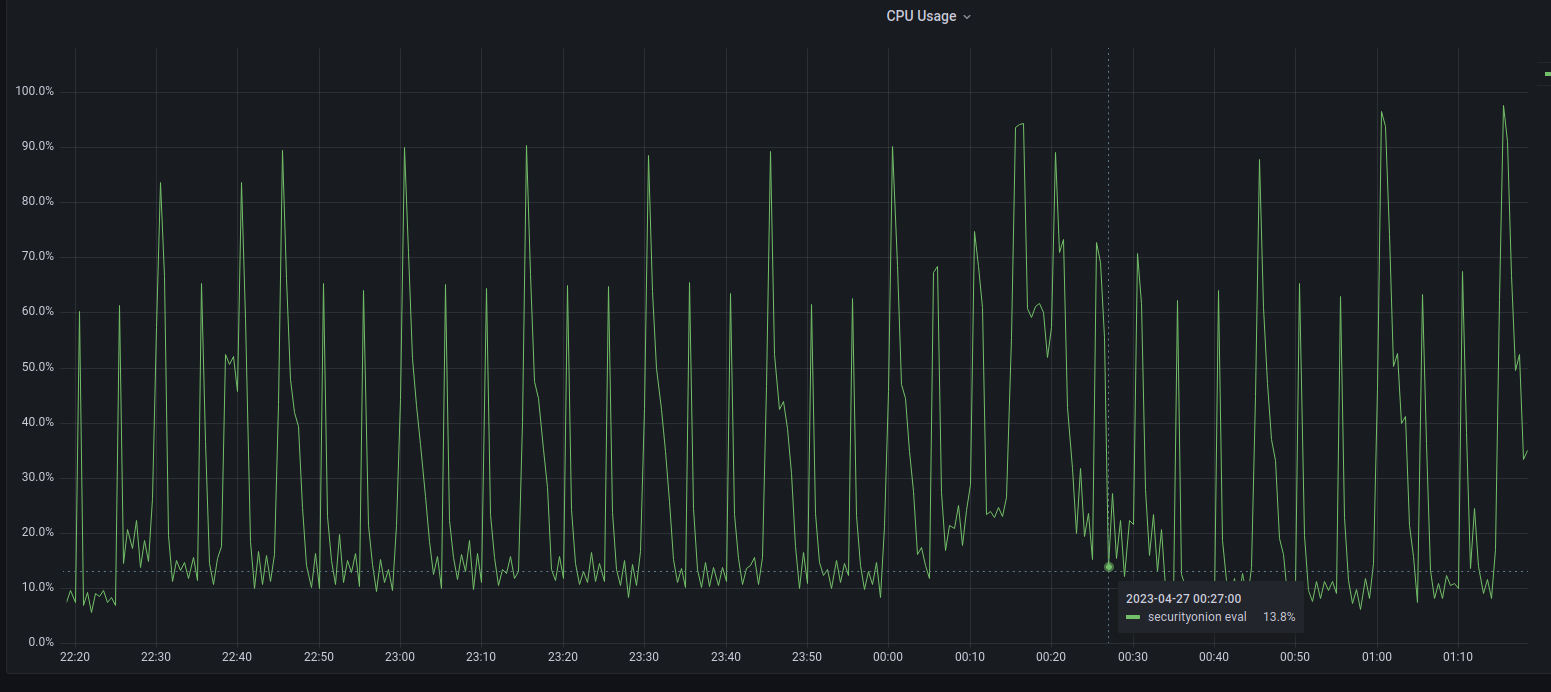
\includegraphics[width=1\linewidth]{CPU1.png}
			\caption{CPU usage when Port-scanning Security Onion take at 00:27 is at 13.8\% } 
			\label{attack1}
			
		\end{figure}
		\end{center}
		
		
		It is evident that the system is not using up all of its resources in this "attack" as this is not a DoS or a DDoS attack, low CPU could be due to point towards many reasons. The most likely reasoning is that Kali's system in this case is only scanning 9 specified ports therefore not much computer resource is used causing the overall workload to be lighter. Other possible reasons include the scanning technique being efficient enough to minimise the overall CPU load through distributing the workload to multiple threads which is a similar concept to Suricata infrastructure in figure \ref{fig:suricata}, to further understand this Nmap scan types can be researched into. 
		
		\begin{center}
		\begin{figure}[H]
			\centering
			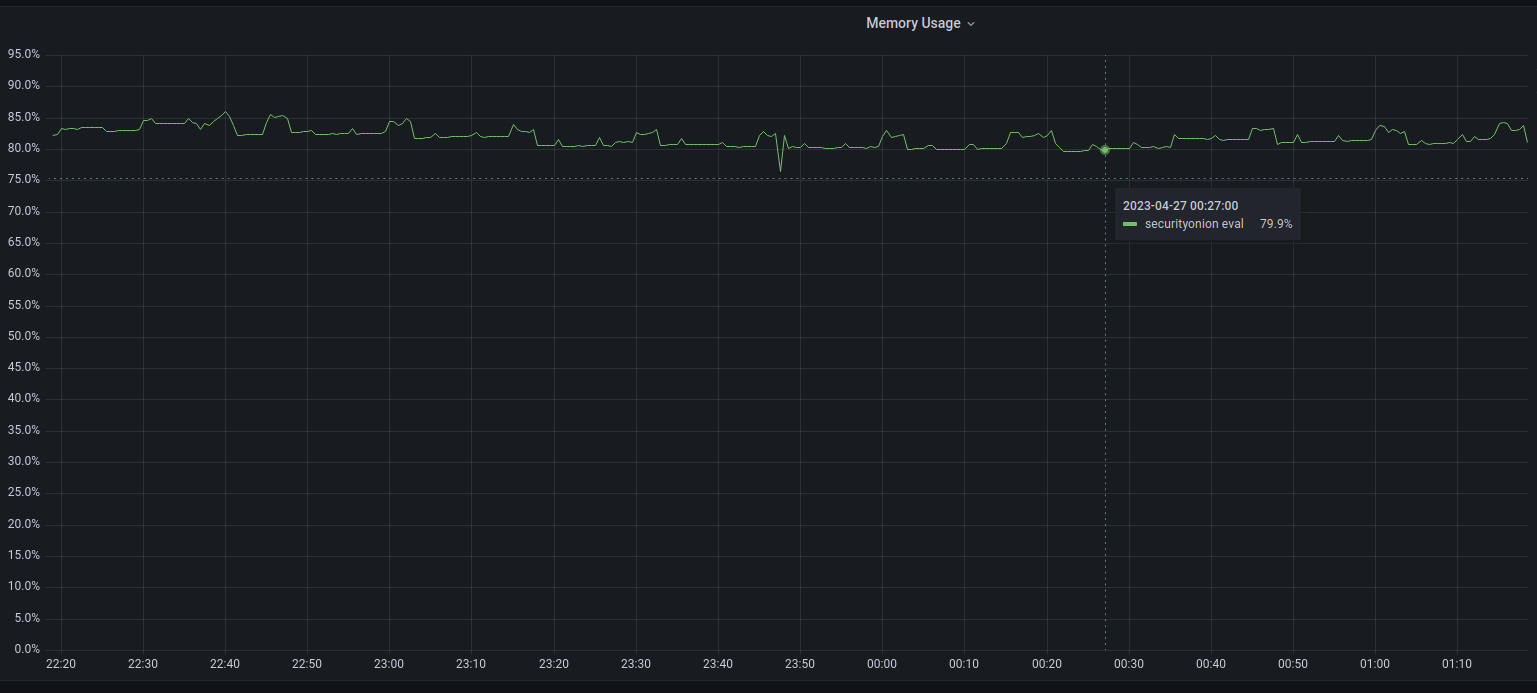
\includegraphics[width=1\linewidth]{MEMORY1.png}
			\caption{Memory usage when Portscanninng Security Onion take at 00:27 is at 79.9\% } 
			
		\end{figure}
		\end{center}
		
		
		Memory usage being 79.9\% is quite high, this could be due to the type of scanning the Nmap is carrying out (TCP and UDP scans) but this cannot be the only contributing factor, it could be Security Onion's role in using the systems resources could be impacting the overall memory usage health.
		
		
		
		\begin{center}
		\begin{figure}[H]
			\centering
			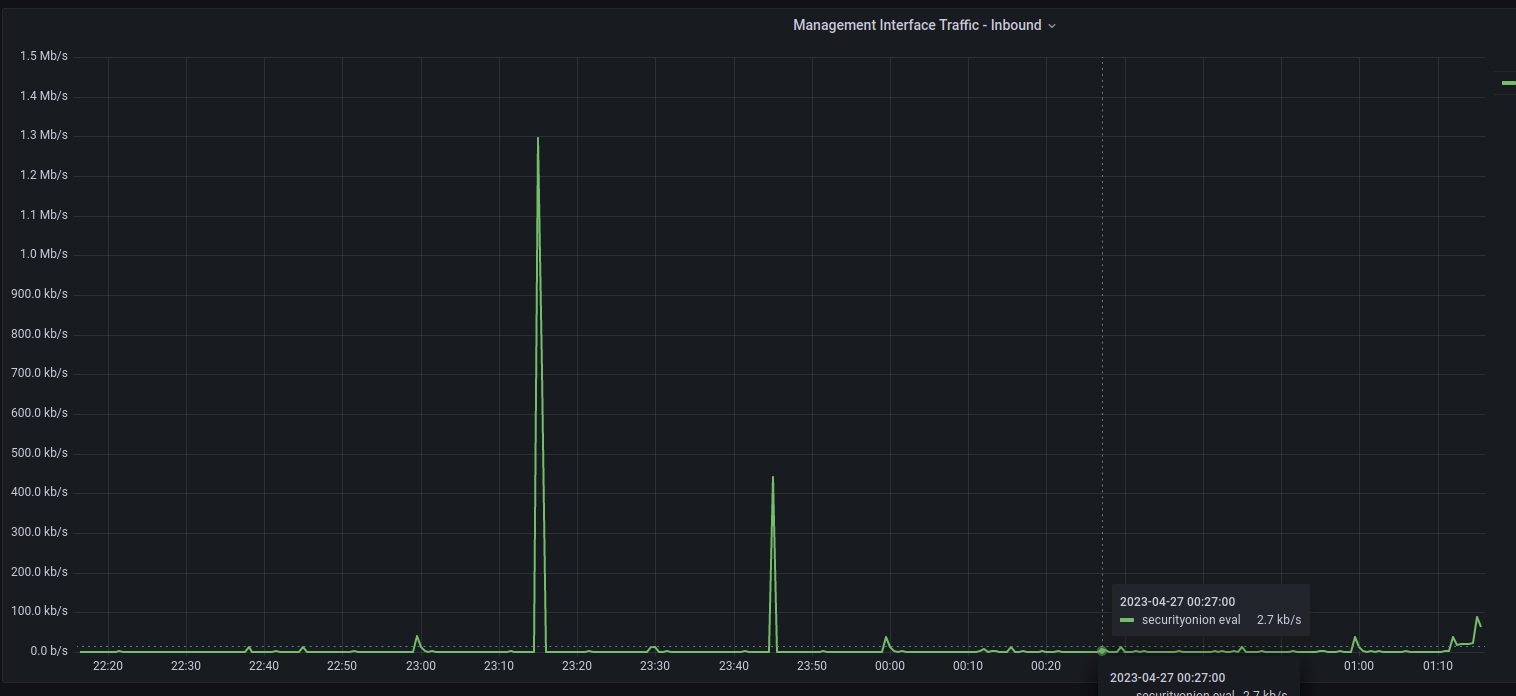
\includegraphics[width=1\linewidth]{Network1.png}
			\caption{The inbound management interface of the network traffic when Portscanninng Security Onion take at 00:27 is at around 2.7 kb/s} 
			\label{fig:attack1}
		\end{figure}
		\end{center}
		
		When it comes to Nmap scanning the packet receiving rate seems to be at 2.7 kb/s, the inbound rate being so low can as stated earlier due to a small range of ports being scanned therefore not impacting network traffic as much.
		
		\begin{center}
		\begin{figure}[H]
			\centering
			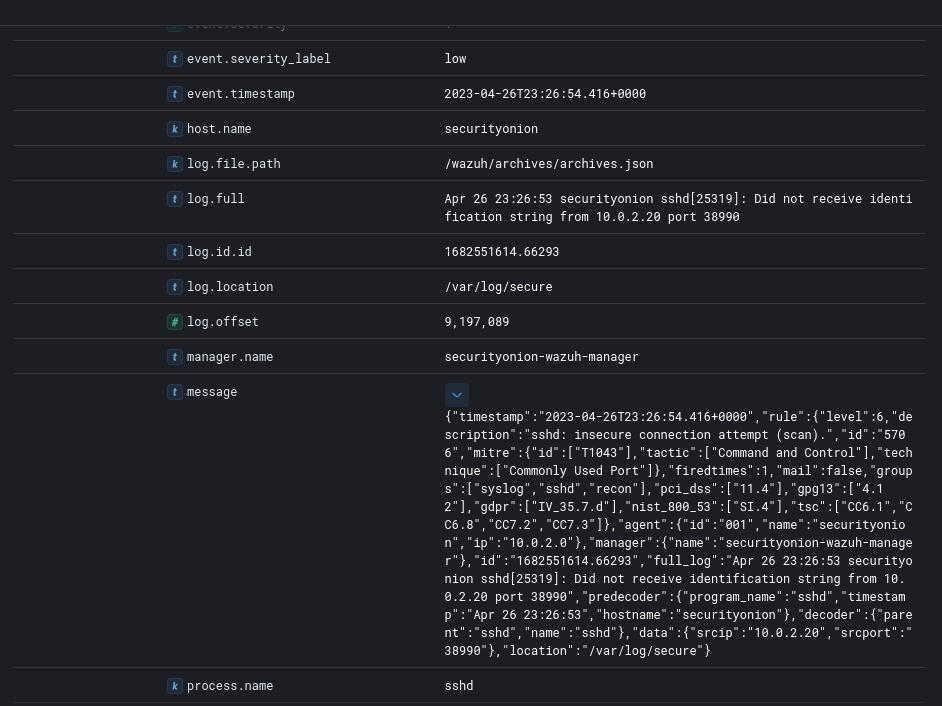
\includegraphics[width=1\linewidth]{threat1.png}
			\caption{Portscanninng Security Onion take at 00:27 } 
			\label{fig:attack1}
		\end{figure}
		\end{center}
		Once the threat is successfully sent from Kali's environment, on the Security Onions console (otherwise known as dashboard) an alert flags up the above message in JSON format. This JSON format attack can be as evidence for the threat in the Security Onion's console. To understand the message from the target address perspective, who has no knowledge of where this attack is coming from only key details will be extracted:
		\begin{itemize}
		\item Timestamp - This conveys when the event of attacks occurred however there is a slight time discrepancy but to briefly speak Kali's environment timing does not match with of Security Onion.
		\item Description -  which is a part of the rule: "6" the number is an indicator of the category the rule falls under in this case the 6 represents the category which this detection fall under, as for the description "sshd - insecure connection attempt (scan)" suggests what kind of detected activity caused the alert to be generated.
		\item MITRE Techniques - which falls under ID "T1043" Points at the technique that is being used by the source IP address.
		\item Compliance Frameworks - "pci\_dss", "gpg13", "gdpr" and "nist\_800\_53" These frameworks are all relevant to the threat received as they fall under different recognised standards and regulations.
		\item Fired Times- refers to the number of times the dashboard flagged this threat.
		\item Source IP and Port - The Source IP and port detected (10.0.2.20 and 38990).
		\item Full Log - refers to additional details the target IP address might find useful.
		
		\end{itemize}
		These details can give the user of the targetted IP address a basic understanding of the attack, specifically the activity that has been detected the attack for, techniques used, the compliance frameworks involved, and lastly any additional details on the source IP and port.
		
		\subsubsection{Brute Forcing SSH login}
		To access a secure communication remotely a malicious user might attempt to infiltrate the system through brute forcing SHH login. This is whereby the attacker tries different combinations of usernames and passwords the victim uses to log into their device. The following command shows how to do so:
		\begin{lstlisting}  [language=bash]
		ssh userid@IPaddress
		\end{lstlisting}
		
		
		\begin{center}
		\begin{figure}[H]
			\centering
			\includegraphics[width=1\linewidth]{ssh.png}
			\caption{Trying multiple passwords to ssh login } 
			\label{fig:34}
		\end{figure}
		\end{center}
		
		In figure \ref{fig:34} the denied permission after every few attempts, has been put in place to delay the brute forcing so that the host system can process the detected activity.
		
		
		In this scenario, the malicious user might use port scanning to extract details about the target IP. Combining port scanning with a brute-forcing tool to guess the password in the case that attacker already knows the username used, gives the attacker a higher chance of gaining unauthorised access. Brute forcing refers to running a script that runs all possible combinations of for example digits or special characters to enter for a password, this is done instead of having to enter manually one by one, this also reduces human error specifically the likelihood of a password combination being missed by chance. 
		To prevent this a user can enforce a strong password policy and use a combination of digits and special characters that makes a password that cannot be linked back to the user behind the target IP address. In addition to this, the Security Onions network intrusion detection system would log this as an alert, as well as deny more than a few attempts each time to log in to limit and delay the multiple attempts to a single target IP.
		
		\subsubsection{UDP attack}
		The concept behind UDP flood attacks has been explained in section \ref{UDP}. But in brief, the attacks overwhelm the system by using up its resources.
		\begin{lstlisting}  [language=bash]
		sudo hping3 --floood -a #.#.#.# -2 -p x #.#.#.#
		\end{lstlisting}
		
		The format for UDP attacks is as follows:
		To understand this low-level threat, "sudo" is necessary as root permission is required to run the command, moving on,hping3 refers to the command tool being used to test the network. The next part of the threat, --flood is an option that comes with hpin3 that causes it to send an immense quantity of packets very fast, moving on to the source IP address the "-a" point at the IP address Kali will flood the Security Onion's system with. The "-2" refers to the UDP option being specified as the transport protocol, the -p is indicating the port that is being entered so in this case the two ports being used are HTTP and SSH. The last set of IP addresses is the target IP address.
		Figure \ref{fig:35} below shows a UDP attack being sent successfully.
		\begin{center}
		\begin{figure}[H]
			\centering
			\includegraphics[width=1\linewidth]{attack2.png}
			\caption{Portscanninng Security Onion take at 18.34 } 
			\label{fig:35}
		\end{figure}
		\end{center}
		Figure \ref{fig:35} below shows a UDP attack being sent successfully, where a total of 13779193 packets have been sent within the span of approximately 45 seconds.
		
		\begin{center}
		\begin{figure}[H]
			\centering
			\includegraphics[width=1\linewidth]{CPU2.png}
			\caption{ Security Onion take at 18.40 } 
			\label{fig:attack1}
		\end{figure}
		\end{center}
		UDP is a transport layer protocol that requires reliable and fast transmissions of packets; hence why it is used for video and voice transmission where all packets are guaranteed to be received.
		As can be seen by the figure above the CPU is at its highest, the most likely reasoning is due to the amount of packets sent for approximately 45 seconds. As this is an amplification attack it is very CPU intensive.
		
		\begin{center}
		\begin{figure}[H]
			\centering
			\includegraphics[width=1\linewidth]{MEMORY2.png}
			\caption{UDP flooding impact on Security Onion's memory usage at around 89.3\% at 18:40:30  } 
			\label{fig:memory2}
		\end{figure}
		\end{center}
		Memory usage is quite high when UDP attacks are sent to the Security Onion. Troubleshooting this accurately requires heavy monitoring of a combination of resources and expertise. High memory usage could be due to memory leaks that have not been released from the memory it has been allocated to, therefore using up more memory than expected. 
		To understand the cause of this better, tools such as SharkTap can be used to assess what is using up memory resources and therefore causing the percentage to be high. It should be noted that the memory usage when port-scanning was also, this may indicate a pattern of tasks taking up memory resources unnoticed rather than a being cause of the attacks.
		
		
		\begin{center}
		\begin{figure}[H]
			\centering
			\subfloat[\centering UDP flooding impact on Security Onion's network inbound usage at around 49.3 kb/s at 18:40:30 ]{{\includegraphics[width=0.45
					\linewidth]{Network2a.png} }}%
			\qquad
			\subfloat[\centering UDP flooding impact on Security Onion's network outbound at around 95.3 kb/s at 18:40:30]{{\includegraphics[width=0.45\linewidth]{Network2b.png} }} 
			\caption{UDP attack's impact on the inbound and outbound network traffic.}
			\label{fig:net}
		\end{figure}
		
		\end{center}
		The inbound traffic graph refers to the amount of data that is required to reply to the attacker's environment (Kali Linux), as for the outbound network traffic graph displays how much data is being sent to the attacker's IP source.
		
		The inbound network traffic being 49.3 kb/s suggests a substantial amount of data is required to be processed, but when compared with the outbound network traffic of 95.3 kb/s, it is a quite good indication that the system handling responding to UDP packets quite well, as there is nearly half of the total packet that requires to be dealt, to put it more simply, Security Onion can send more processed data out than it is receiving.
		
		Taking preventative measures is still necessary to protect the system's integrity, a solution to this can be to immediately terminate the connection between the system and network.
		
		
		
		\subsubsection{TCP SYN Flood Attack}
		
		The penultimate attack that will be tested on Security, occurs when the attacker initiates a connection but never responds, creating a backlog of unanswered messages in Security Onion's system therefore using up its resources.SYN packets are what are used to establish connections.
		
		\begin{lstlisting}  [language=bash]
		sudo hping3 #.#.#.# -q -n -d 120 -S -p 80 --flood --rand-source
		\end{lstlisting}
		
		The format for TCP SYN flood attacks is as follows:
		To understand this low-level threat, "sudo" is necessary as root permission is required to run the command, moving on, hping3 refers to the command tool being used to test the network. The hashes represent the target IP address, and "-q" stands for quiet which suppresses the amount being displayed. The -n is a numeric value used to disable the DNS server, by doing so it is ensure that the hping3 command uses the target IP without trying to mitigate unresolved hostnames. The next part involves "-d 120" which refers to the data size per each packet to be a total of 120 bytes filled with randomise data. Moving on to the "-S" set the packets to indicate that they 
		TCP SYN packets,  the "-p" is indicating the port that is being entered so in this case the port being used is HTTP. The --flood is an option that comes with hpin3 that causes to send packets of data continuously, and lastly --rand-source refers to spoofing the source IP address to make it harder to identify the attacker's address.
		
		\begin{center}
		\begin{figure}[H]
			\centering
			\includegraphics[width=1\linewidth]{syn1.png}
			\caption{TCP SYN flooding impact on Security Onion's target IP address 21:09  } 
			\label{fig:syn1}
		\end{figure}
		\end{center}
		After successfully sending this attack it should be noted that there was a two-minute delay right after in Kali's system this could be due to Kali not finishing sending the attack, and it further skewed the results as the JSON logs do not specify the activity detected are related to the attack.
		To identify this attack approximate timestamps were used as the attack was not flagged in the alert section.
		
		
		\begin{center}
		\begin{figure}[H]
			\centering
			\includegraphics[width=1\linewidth]{cpusyn.png}
			\caption{TCP SYN flooding impact on Security Onion's CPU usage at around 54.6\% at 21:09  } 
			\label{fig:memory2}
		\end{figure}
		\end{center}
		
		As it can be seen the attack seems to have little impact on CPU usage, there could be many reasoning however it should be noted moments after this the next peak in the graph is much higher, one possible reason for this is network latency, as although a substantial amount of packets are being sent they are being sent a few minutes later than they should. The cause for this may be the packet size of 120 bytes impacting the transportation protocol layer.
		
		
		\begin{center}
		\begin{figure}[H]
			\centering
			\subfloat[\centering TCP SYN  flooding impact on Security Onion's network inbound usage at around 51.6 Mb/s at 21:09 ]{{\includegraphics[width=0.45
					\linewidth]{inboundsyn.png} }}%
			\qquad
			\subfloat[\centering TCP SYN  flooding impact on Security Onion's network inbound usage at around 9.7 Mb/s at 21:09]{{\includegraphics[width=0.45\linewidth]{outboundsyn.png} }} 
			\caption{UDP attack's impact on the inbound and outbound network traffic.}
			\label{fig:net1}
		\end{figure}
		
		\end{center}
		
		This attack processed greater quantities of both inbound and outbound network traffic compared to the previous attack which can be referred back to \ref{UDP}. Comparing inbound and outbound suggests that more data is being received to be processed than packets of data that have already been processed and are ready to be sent back. If this situation escalates Security Onion's system can potentially crash. 
		A way to prevent this would be to implement Intrusion Prevention System (IPS), which is used to not only detect malicious activity but also prevent attacks from occurring. 
		
		
		
		\subsubsection{ICMP attack}
		The last attack involves masking as the target address to echo to a network of IP addresses which echo back to the real target IP address flooding the system with replies, this attack has been covered in more depth in section \ref{ICMP}
		\begin{lstlisting}  [language=bash]
		sudo hping3 #.#.#.# -q --ICMP -C 3 -K 4 --faster
		\end{lstlisting}
		
		
		The format for UDP attacks is as follows:
		To understand this low-level threat, "sudo" is necessary as root permission is required to run the command, moving on, hping3 refers to the command tool being used to test the network. The next part of the threat, "-q" stands for quiet which suppresses the output that is being displayed. The "--ICMP" is an option that comes with hping3 that causes specifically ICMP packets to be sent. "C 3" refers to the number of echo request packets that are to be sent which means 3 echoed replies will be sent to the target IP. Moving onto "-K 4 ", this simply acts as an identifier. And lastly, --faster is a command for a faster process preventing any possibilities of delay.
		\begin{center}
		
		\begin{figure}[H]
			\centering
			\includegraphics[width=1\linewidth]{ICMP.png}
			\caption{ICMP attack's impact on Security Onion at 00:45:33 lasting around 2 minutes. } 
			\label{fig:memory2}
		\end{figure}
		\end{center}
		For this attack, the focus has been on the dashboard's result. Whilst understanding the health of the system in the precious attacks, the detection performance on the dashboard had been slightly overlooked. The result of this attack did not display any indication of the source address, the only way to identify the alert from the attack was by matching the timestamps, on the JSON log system the following two messages were displayed:
		\begin{lstlisting} [language=json,firstnumber=1 ,escapeinside={(*}{*)}, numbers=left]
		"note":"CaptureLoss::Too_Little_Traffic",
		"msg":"Only observed 0 TCP ACKs and was expecting at least 1."
		(*\textcolor{red}{\footnote{The note and the message}}*) \end{lstlisting} 
		
		Although other attacks were timed to be at 45 seconds, due to the message suggesting the threat did not occur for long enough, this attack was carried out a second time for a lengthy period of two minutes, the log for this was the same, which based on the following log :
		
		
		
		\begin{lstlisting} [language=json,firstnumber=1 ]
		"actions":["Notice::ACTION\_LOG"],"email\_dest":[],"suppress\_for":3600.0}
		
	\end{lstlisting} 



suggested the engine detecting this threat Zeek might have been configured to suppress this form of alert in its rule file.


\section{Discussion and Evaluation}
\subsection{Objectives}
The following objectives were proposed at the start of the project:
\begin{itemize}
\item To study different forms of network threats. This has been done in the literature review section of this report beginning from section \ref{3.1}.
\item To design and analyse the implementation of a simulated network. This objective has been changed for a more realistic experiment, the initial idea entailed using software to send attacks to a cluster of devices. Instead, virtual machines are being used where configurations can be manipulated better. 
\item To implement Security Onion as a proxy, this objective has also been changed to fit a more realistic experience whereby Security Onion's virtual machine is used as a target address and there was no need to fit it as a proxy due to the environment already having multiple NIDS embedded in the system.
\item To examine Security Onion implemented in the simulated network. This objective has been completed, it starting from section \ref{testing}.
\item To evaluate how Suricata recognises network threats, although the understanding of Suricata's role has been refined and explored throughout the report, it is a combination of Suricata Snort and Zeek that are embedded within the system however only one can be used at a time, according to the documentation one NIDS has to be disabled before another can be enabled. The focus of this objective has shifted towards evaluating how effective Security Onion is at detecting unusual activities.
\item To conclude on the effectiveness of Security Network to detect network intrusions. This objective has been achieved successfully.

\end{itemize}

\subsection{Amended issues}
This section focuses on issues that have been encountered during the completion of this project and have been rationalised.

\subsubsection{Time discrepancy}
An important note to be made in this report is that there is a one-hour time discrepancy. Where the Kali Linux is set to Europe/London time, the Security Onion is set one hour back from that. This can be easily fixed through the date command by doing sudo timedatectl set-timezone YOUR\_COUNTRY. The Security Onion Documentation, however, advises not to change this one-hour setback as this (UTC/GMT)timing can be used to correlate different cybersecurity events within systems across the world and therefore not changing this time zone is considered as best practice within the industry.
\subsubsection{Sudo Crash}
Users who may be using the file attached to this document must be aware of sudo crashing, this can be due to a long period of inactivity creating a backlog of necessary updates, while executing this project, this issue was faced and the only viable solution was to reinstall the Security Onion's environment as going into recovery mode to repair the sudo command was not an option. Therefore consistently updating both environments is necessary to avoid such problems.

\subsection{False Positives}
A lot of alerts in the dashboard consisted of false positives such as NAT detections, which can lead to unwanted skews in graphs causing other attacks to go unnoticed, to suppress false positives according to the Security Onions's documentation the rules can be tuned. Numbers are used as an indication of the severity level used by the engines Suricata, Wazuh, and Playbook. The severity is categorised as follows:
\begin{itemize}
\item event.severity: 4 ==>  event.severity\_label: critical
\item 	event.severity: 3 ==> event.severity\_label: high
\item	event.severity: 2 ==> event.severity\_label: medium
\item	event.severity: 1 ==> event.severity\_label: low


\end{itemize} 
For instance, Wazuh, a host-based intrusion detection system responsible for detecting unusual activities giving a lot of false positives can be modified by including a noalert="1" in the rule section.
\subsection{Further Development}

There are alternative methods that are far more ideal compared to portscan, instead of using Nmap, using the GUI version called Zenmap would mean that a wider range of ports would be port-scanned instead of a few randomly selected port numbers. 

To further understand the very powerful engines embedded within Security Onion one can compare their detection algorithms in a controlled environment, this could have been done in this project however due to time constraints it is not possible, this is because Security Onion requires enabling and disabling each time the preferred engine is changed and for multiple attacks with multiple trials this was not an option.

To further explore this in this project only low-level attacks have been carried out due to insufficient expertise in this field, this research can be further pushed by carrying out higher-level attacks to imitate real threats better.

\subsection{Conclusion}

To conclude this report, Security Onion is an effective and easy-to-use NIDS solution that offers several unique advantages over other systems. Its simplicity and ease of use make it an attractive option for organisations looking to improve their network security. Its scalability and its powerful security tools make it an effective tool for detecting and responding to network intrusions. However, this framework requires much more research and testing to ensure it is as mentioned in the initially proposed concern; whether Security Onion is an effective distribution.

All research done so far on Security Onion are experiments implemented using an older version of Security Onion. The experiments have carried an updated version of Security Onion, the latest version being 2.3.200, however to ensure a stable version has been used in this project. The version suggested at the front of the Security Onion's website has been used instead. Using an updated distribution makes this a fresh research with potentially newer and higher results in terms of accuracy. More research involving a broader spectrum of attacks is required to conclude, as this project mainly focused on DoS/DDos-based attacks. 

An overall theme to be noted is where a low-level flooding-based attack gets little relevance in the dashboard alert, in the same manner, short burst low-level threats get flagged under alerts suggesting that Security Onion's default configuration focuses on efficiency as logging packets sent every millisecond would greatly impact the system's memory instead it records how many times the attack has been fired within that short window of time. To better this every user deems efficiency differently, not much reconfiguration is required to use SO, therefore, it may be suitable for users who are not experienced in using Security Onion as their Operating system. The next steps in the research implementation of this project involve using real severe attacks in controlled settings to understand where Security Onion's limitations fall.




\section{User Guide} \label{userguide}
This section is going to be a user-friendly guide to allow individuals with access to the .vdi files to carry out the same attacks to test security onion in their environment.

To commence, there will be two .vdi files that will be attached along with this documentation. One of the fie is to run the security onion environment that has been ready set up and the latter is for Kali. If Virtual Box has not already been installed, the user would simply need to:
\begin{itemize}
\item Set the name and folder path for the virtual environment.
\item Choose the type of Linux distribution version that is going to be used.
\item Make decisions on storage and CPU  based on their machine's capability.
\end{itemize} 
After doing so, within the VirtualBox (VBox) manager interface such as in figure \ref{18a} which displays all the machines running, under storage there should be an option to create or upload personal disk files. 
Here the user should choose their own.

This should enable them to run both environments without setting up any of the initial steps in deploying virtual machines.

A few important things required to be noted when running these machines are listed below:
\begin{itemize}
\item Security Onion's IP address (Target IP)- 10.0.2.0
\item Kali Linux's IP address (Source IP)- 10.0.2.20
\item The username for both environments- silvia 
\item The password for both environments silvia123
\item The username for Security Onions Console that is accessed through Kali Linux's browser- SA3046@live.mdx.ac.uk
\item The password for security onion's console- silvia123 
\item The username to Grafana should be as stated by the documentation- admin
\item The password for Grafana is- 4bav4b5thBn4Qk2kJiWm
\end{itemize}

To access Security Onion's dashboard within the Kali Linux environment, a command would be required to be run if it's the first time and will be required every once in a while, the user would be required to allow the IP range to be allowed to view the analytics. To do this the user would run the following command as the root.



\begin{lstlisting}[language=bash]
sudo so-allow
\end{lstlisting}

the user then should select the purpose, in this project a) analytics was chosen, and sequentially the user will be prompted the IP address to allow viewing the dashboard (In this case it should be Kali's). If sudo does not work it might be that Security Onion's configurations are not updated. There are cases in which going into recovery mode does not resolve the issue, if this is the case the user needs to redeploy the security onion from the start. Therefore it is suggested the user looks out for necessary updates. The Security Onion .vdi file attached is just a command prompt hence why it is necessary to be able to have access to the dashboard and this can be done so by accessing Linux's environment. This step is done to ensure the dashboard is ready to be viewed, the following command should display an [ok] on each container similar to figure \ref{32b} :
\begin{lstlisting}  [language=bash]
sudo so-status
\end{lstlisting}
When all containers are "OK", the user can then proceed to open any browser in Kali and enter Security Onion's IP address. If prompted to enter login details the user should enter the email and password entered when configuring Security Onion, an example of doing this can be viewed in figure \ref{31b}.

To make a health check on the Security Onion's environment, the user can Grafana which has been made available on the dashboard however the username and password are different. According to the documentation the username is set to "admin", and as for the password can be accessed through the following command:
\begin{lstlisting}  [language=bash]
sudo salt-call pillar.get secrets 
\end{lstlisting}


\begin{center}
\begin{figure}[H]
\centering
\includegraphics[width=1\linewidth]{cpu.png}
\caption{Security Onion's health overview viewed through Grafana. } 
\label{fig:attack1}
\end{figure}
\end{center}

If for any reason the command above cannot be used to retrieve the password for Grafana's health overview dashboard, the user can use htop to view the CPU from the command line in the case that the command line Security Onion is being used rather than GUI.






	\section{References }
	
	\renewcommand{\bibsection}{}
	
	\bibliographystyle{unsrt}
 
	\bibliography{reference3}
	
		\section{Appendices}
	\subsection{Brute Forcing SSH login}
	\begin{lstlisting}[language=json,firstnumber=1]	
		{"timestamp":"2023-04-23T20:16:59.103+0000","rule":{"level":5,"description":"sshd: authentication failed.","id":"5716","mitre":{"id":["T1110"],"tactic":["Credential Access"],"technique":["Brute Force"]},"firedtimes":3,"mail":false,"groups":["syslog","sshd","authentication_failed"],"pci_dss":["10.2.4","10.2.5"],"gpg13":["7.1"],"gdpr":["IV_35.7.d","IV_32.2"],"hipaa":["164.312.b"],"nist_800_53":["AU.14","AC.7"],"tsc":["CC6.1","CC6.8","CC7.2","CC7.3"]},"agent":{"id":"001","name":"securityonion","ip":"10.0.2.0"},"manager":{"name":"securityonion-wazuh-manager"},"id":"1682281019.25850","full_log":"Apr 23 20:16:59 securityonion sshd[29364]: Failed password for silvia from 10.0.2.20 port 50528 ssh2","predecoder":{"program_name":"sshd","timestamp":"Apr 23 20:16:59","hostname":"securityonion"},"decoder":{"parent":"sshd","name":"sshd"},"data":{"srcip":"10.0.2.20","srcport":"50528","dstuser":"silvia"},"location":"/var/log/secure"}
	\end{lstlisting}
	
	\section{Ethics Approval}
	\includepdf[pages=-]{ethics.pdf}
\end{document}